% ICDE preview assembled from the supplied IEEE conference template.
% Independent English section copies; the NDSS manuscript is unchanged.
% Compile from this directory: latexmk -pdf icdever.tex
\documentclass[conference]{IEEEtran}
\IEEEoverridecommandlockouts
\usepackage[T1]{fontenc}
\usepackage{amsmath,amssymb,amsfonts,amsthm}
\usepackage{cite}
\usepackage{graphicx}
\usepackage{textcomp}
\usepackage[table]{xcolor}
\usepackage{booktabs,multirow,tabularx}
\usepackage{pifont}
\usepackage{tikz}
\usepackage[caption=false,font=footnotesize]{subfig}
\usepackage{float}
\usepackage{placeins}
\usepackage[ruled,linesnumbered]{algorithm2e}
\usepackage[hidelinks]{hyperref}
\usepackage{cleveref}
\newtheorem{theorem}{Theorem}
\newtheorem{definition}{Definition}
\newtheorem{lemma}{Lemma}
\newtheorem{proposition}{Proposition}
\newcommand{\red}[1]{\textcolor{red}{#1}}
\newcommand{\blue}[1]{\textcolor{blue}{#1}}
\newcommand{\vsvar}{1mm}
\newcommand{\draftplaceholder}{\textcolor{blue}{xxx}}
\newcommand{\gddmissing}{\draftplaceholder}
\newcommand{\gddvaluesfile}{icde_sections/experiment_values.tex}
\Crefname{equation}{Eq.}{Eqs.}
\crefname{algorithm}{algorithm}{algorithms}
\Crefname{algorithm}{Algorithm}{Algorithms}
\crefname{algocf}{algorithm}{algorithms}
\Crefname{algocf}{Algorithm}{Algorithms}


\usepackage{graphicx}
\usepackage[caption=false,font=footnotesize]{subfig}

\begin{document}
\title{PrivTDD: Triangle-Degree Distribution Estimation under Edge-Local Differential Privacy}
% \author{\IEEEauthorblockN{Beibei Cheng}
%   \IEEEauthorblockA{\textit{Southeast University}\\
%     Nanjing, China\\
%     bbcheng@seu.edu.cn}
%   \and
%   \IEEEauthorblockN{Kai Dong}
%   \IEEEauthorblockA{\textit{Southeast University}\\
%     Nanjing, China\\
%     dk@seu.edu.cn}
%   \and
%   \IEEEauthorblockN{Yuanbo Zhao}
%   \IEEEauthorblockA{\textit{Southeast University}\\
%     Nanjing, China\\
%     zhaoyb@seu.edu.cn}
%   \and
%   \IEEEauthorblockN{Jingbo Sun}
%   \IEEEauthorblockA{\textit{Southeast University}\\
%     Nanjing, China\\
%     jingbosun@seu.edu.cn}
%   \and
%   \IEEEauthorblockN{Guangchi Liu}
%   \IEEEauthorblockA{\textit{Southeast University}\\
%     Nanjing, China\\
%     xxx@seu.edu.cn}
%   \and
%   \IEEEauthorblockN{Zhen Ling}
%   \IEEEauthorblockA{\textit{Southeast University}\\
%     Nanjing, China\\
%     zhenling@seu.edu.cn}}
\author{
\IEEEauthorblockN{
Beibei Cheng, Kai Dong, Yuanbo Zhao,
Jingbo Sun, Guangchi Liu, Zhen Ling
}
\IEEEauthorblockA{
\textit{School of Computer Science and Engineering, Southeast University,} Nanjing, China
\\
\{bbcheng, dk, zhaoyb, jingbosun, gc-liu, zhenling\}@seu.edu.cn
}
}
\maketitle
\begin{abstract}

% The \textbf{triangle degree distribution (TDD)} records how many nodes have each triangle participation count, revealing participation heterogeneity.
% Under edge-local differential privacy, users generally cannot observe edges among their neighbors, making participation counts locally unavailable.
% Directly binning noisy estimates can distort the histogram even when the global triangle count is accurate.
% We introduce PrivTDD, which decomposes TDD recovery into a \textbf{wedge-count distribution} (neighbor-pair counts) and \textbf{degree-conditioned closure-rate distributions} (fractions of neighbor pairs that are connected).
% Wedge counts depend only on locally known degrees and can be estimated from privatized degree reports without inferring triangle counts.
% Modeling closure-rate distributions instead pools noisy relational evidence across nodes.
% PrivTDD constructs complementary structural references capturing degree heterogeneity and local clustering, then learns regional mass and within-region shape corrections from private reports using the known reporting mechanism.
% Posterior reweighting and probabilistic aggregation yield a candidate TDD estimate.
% We establish privacy and utility guarantees and derive a budget allocation minimizing the resulting error bound.
% Across four real networks and eight privacy budgets, PrivTDD achieved the lowest mean earth mover's distance in 30 of 32 settings, including a 90.6\% reduction on DBLP at $\varepsilon=2$ (2.65 versus 28.24 for the best baseline).
% Artifacts are available at \url{https://github.com/Luna-iris/PrivTDD}.
The \textbf{triangle-degree distribution (TDD)} counts nodes by triangle degree, the number of triangles containing a node. Under edge-local differential privacy, users generally cannot observe edges between their neighbors. Binning noisy triangle-degree estimates can distort the TDD despite accurate global triangle counts.
PrivTDD decomposes TDD estimation into a \textbf{wedge-count distribution} (neighbor-pair counts) and \textbf{degree-conditioned closure-rate distributions} (fractions of connected neighbor pairs). It estimates the former from privatized degree reports and models the latter by pooling noisy reports across nodes.
Two structural models predict reference distributions reflecting degree heterogeneity and local clustering. Private reports guide adjustments to probabilities across and within count ranges. PrivTDD then updates count probabilities using each node's reports and aggregates across node degrees into a candidate TDD estimate.
We prove privacy guarantees and derive a budget allocation minimizing the bound. Across four real networks and eight privacy budgets, PrivTDD achieves the lowest mean earth mover's distance (EMD) in 30 of 32 settings, including a 90.6\% reduction on DBLP at $\varepsilon=2$ (2.65 versus 28.24 for the best baseline).
Artifacts are available at https://github.com/Luna-iris/PrivTDD.

\end{abstract}
\begin{IEEEkeywords}
Local differential privacy, triangle-degree distribution, graph analytics.
\end{IEEEkeywords}
\section{Introduction}
\label{sec:introduction}
% Faithful translation of the existing Chinese introduction.
Graph analysis under local differential privacy (LDP) has become an important research direction in graph data analytics.
These techniques aim to enable an untrusted server in a distributed setting to perform graph-structure statistics and analysis without exposing users' private information, including private edges or adjacency information.
Existing studies have developed basic graph analysis operators for node degrees and subgraph counting~\cite{imola2021locally,Ye2022}.
However, existing LDP graph analysis operators primarily target node-level scalar statistics or global structural counts, rather than the \textbf{triangle degree distribution (TDD)}. %
Triangle degree counts the triangles containing a node; the TDD counts nodes with each triangle degree.
Compared with node degrees or global triangle counts, which reflect local connectivity or overall triangle abundance, TDD preserves information on local triangle participation and its heterogeneity across nodes~\cite{becchetti2008local,antunes2021sampling}.
TDD therefore serves as an important structural statistic for graphlet-based network comparison~\cite{LDPGDDPrzulj2007,hayes2013graphlet} and as an input for graph generation~\cite{zahirnia2023neural}.
% TDD therefore provides a useful structural descriptor for network comparison and the characterization and modeling of clustered network structures~\cite{LDPGDDPrzulj2007,pham2024clustering}.


% Graph analysis under local differential privacy (LDP) has become an important research direction in graph data analytics.
% These techniques aim to enable an untrusted server in a distributed setting to perform graph-structure statistics and analysis without exposing users' private information, including private edges or adjacency information.
% Existing studies have developed basic graph analysis operators for node degrees, triangle counting, and subgraph counting~\cite{imola2021locally,Ye2022}.
% However, existing LDP graph analysis operators primarily target individual scalar statistics or a small number of global structural counts, and cannot yet support operators such as the \textbf{triangle degree distribution (TDD)}.
% TDD characterizes the frequency distribution of the numbers of higher-order graphlets in which nodes or edges participate.
% Compared with scalar statistics such as node degrees or global triangle counts, which reflect only local connectivity or overall closure, TDD preserves richer local structure and its heterogeneity across nodes~\cite{faloutsos1999power,tsourakakis2008fast,sphICDM}.
% TDD therefore offers greater structural expressiveness and supports a broader range of applications, including network comparison, motif identification, anomalous topology detection, and biological and financial network analysis~\cite{motifs,subgraphTopolgy,LDPTDDPrzulj2007,wegner2018identifying,yoon2023graphlets,elliott2019anomaly}.

Existing techniques cannot adequately support an  applicable TDD operator under LDP, as illustrated in Fig.~\ref{fig:tdd-motivation}\subref{fig:tdd-limitation}.
As with existing LDP operators, implementing a TDD operator requires both local randomized reporting and server-side aggregation and estimation~\cite{LDPGDDWang2017,imola2021locally}, and its central difficulties arise in both stages.
First, during local randomized reporting, users must randomize and report the private quantity to be aggregated, namely their triangle degree.
However, in the TDD task under distributed privacy constraints, each user does not know this value in advance.
% Using existing LDP techniques, \textbf{estimating this unknown scalar introduces additional error}, because each user must perform an LDP-compliant aggregation and recovery procedure to obtain it.
Using existing LDP techniques, \textbf{estimating this locally unknown scalar introduces additional error}, as it requires inferring triangle degrees from noisy information about edges.
Second, during server-side aggregation and estimation, the TDD operator must estimate a histogram of triangle degrees rather than a single scalar statistic. %the complete distribution of graphlet degrees, typically represented as a histogram, rather than a simple scalar statistic.
Directly applying existing LDP techniques to \textbf{estimate this high-dimensional distribution further amplifies the additional error introduced in the preceding stage}.
% Taking \draftplaceholder{} as an example, the procedure first \draftplaceholder{} and then assigns nodes to the corresponding histogram bins according to their locally randomized reported values.
For example, LDPGraph estimates triangle degrees from privatized graph reports~\cite{dong2026ldpgraph}.
A direct TDD adaptation would discretely bin these estimates.
Unlike linear aggregation tasks such as global triangle counting, where positive and negative errors may cancel in summation, such binning can shift nodes between bins and distort the histogram, especially under tighter privacy budgets.
% Unlike linear aggregation tasks such as global triangle counting, however, TDD requires discrete binning before aggregation.
% Unlike global triangle counting, where positive and negative numerical errors may cancel during summation, such binning can move nodes between histogram bins, distorting their frequencies.
% Consequently, noise introduced by the LDP mechanism cannot cancel out through aggregation into a single scalar statistic, instead, it is distributed across histogram bins. %and manifests as mass migration between bins.
% The estimation error in the previously unknown scalar is thus further transformed into additional distributional distortion.
% In particular, under stronger privacy constraints, greater uncertainty in recovery further increases such cross-bin errors.
%the probability of nodes crossing bin boundaries, ultimately producing substantial TDD distortion.

% \begin{figure}[t]
%   \centering
%   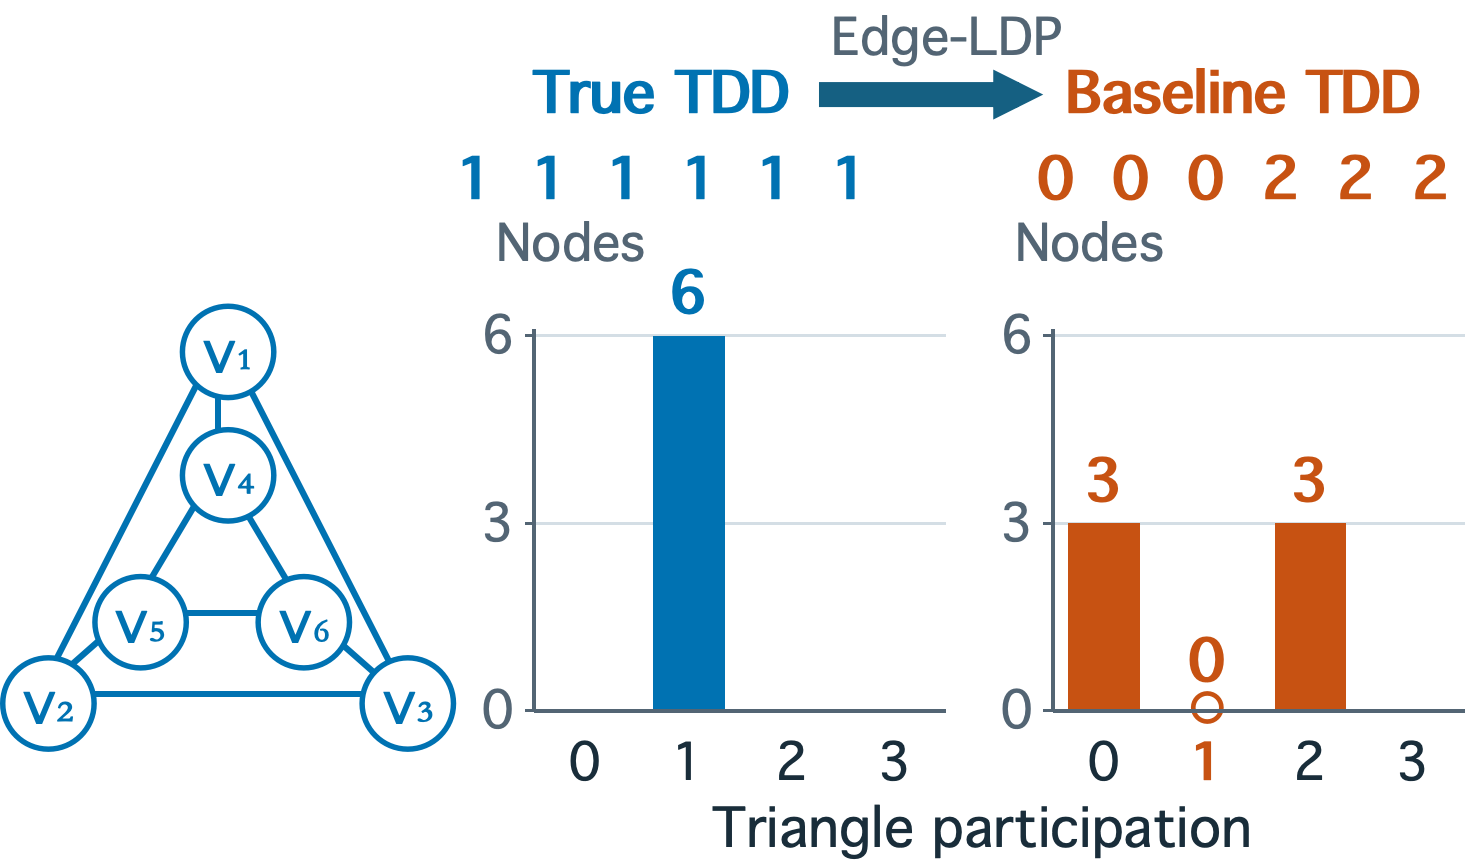
\includegraphics[trim=0mm 0mm 0mm 0mm,clip,width=\linewidth]{icde_sections/limitation.png}
%   \caption{Limitations of baseline composed by existing LDP operators.}
%   \label{fig:limitation}
% \end{figure}

% \begin{figure}[t]
%   \centering
%   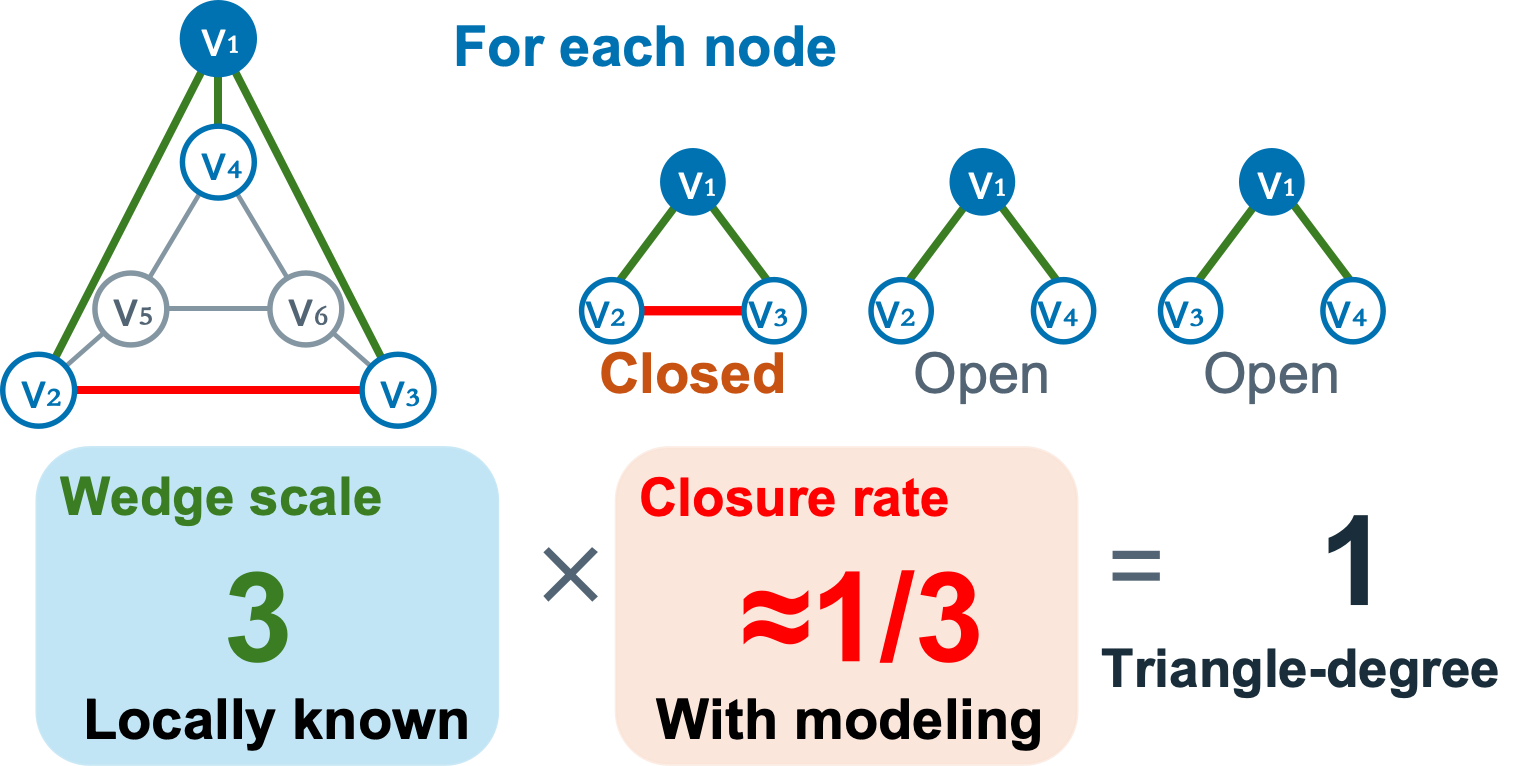
\includegraphics[trim=0mm 0mm 0mm 0mm,clip,width=\linewidth]{icde_sections/basic idea.png}
%   \caption{Basic idea of PrivTDD.}
%   \label{fig:basic_idea}
% \end{figure}


\begin{figure}[t]
    \centering
    \subfloat[Limitation of existing techniques]{
        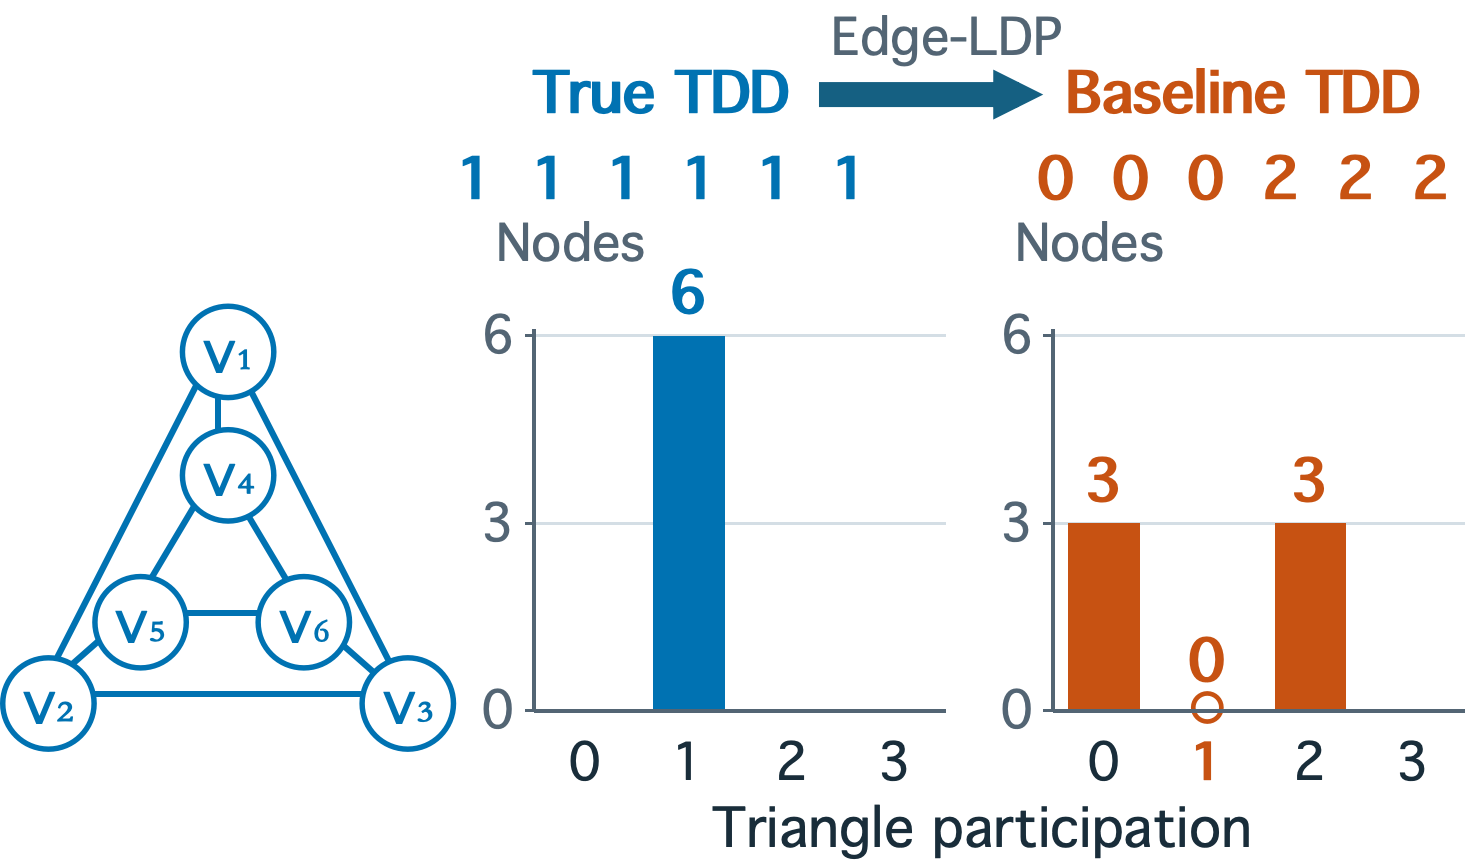
\includegraphics[width=0.45\columnwidth]{icde_sections/limitation.png}
        \label{fig:tdd-limitation}
    }
    \hfill
    \subfloat[Basic idea]{
        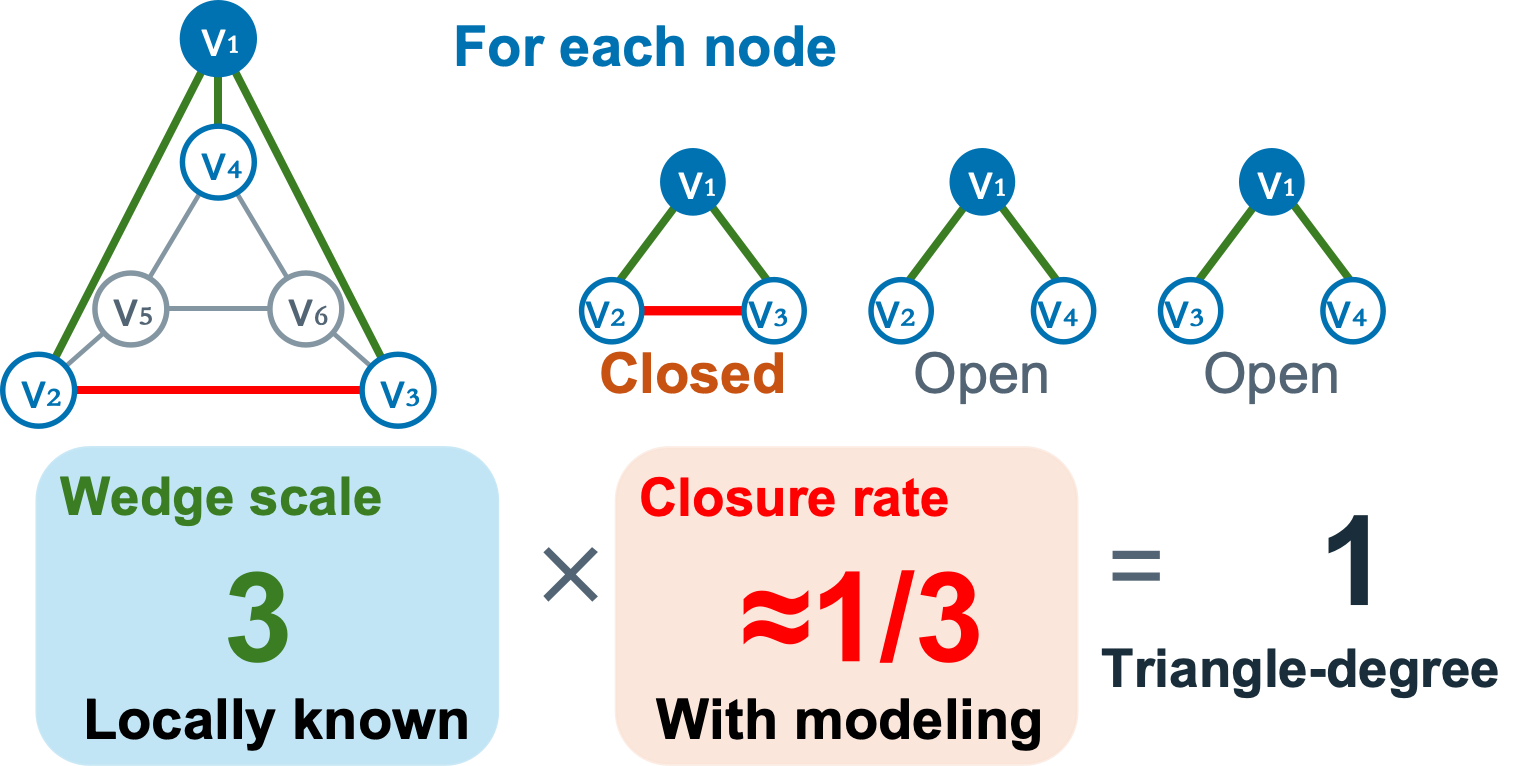
\includegraphics[width=0.45\columnwidth]{icde_sections/basic idea.png}
        \label{fig:tdd-basic-idea}
    }
    \caption{(a)  Existing techniques cannot support an applicable TDD operator under LDP, since binning noisy triangle-degree estimates can distort the TDD despite an accurate global triangle count.
    (b) Our basic idea is to decompose triangle-degree estimation into wedge-count and closure-rate (red) estimation.}
    \label{fig:tdd-motivation}%todo
\end{figure}


This paper proposes the first TDD operator under LDP, \textbf{PrivTDD}.
Its central idea is to transform the complex TDD estimation operator into a combination of two simpler estimation operators.
Specifically, instead of computing the TDD by assigning triangle degree values to different histogram bins, the method decomposes direct TDD estimation into modeling the distributions of \textbf{wedge counts} and \textbf{closure rates} (as illustrated in Fig.~\ref{fig:tdd-motivation}\subref{fig:tdd-basic-idea}).
A node has one wedge per neighbor pair; its closure rate is the fraction connected. This decomposition provides two benefits.
First, and more directly, estimating the wedge-count distribution introduces little error.
Although this remains a high-dimensional histogram estimation task, it only aggregates wedge counts, which users already know, rather than triangle degrees, which they do not.
The resulting error is therefore much smaller than the error involved in estimating an unknown quantity, avoiding the additional two-stage error amplification described above.
The second benefit is more subtle.
Estimating closure rates through LDP alone does not yield more accurate estimates, because the closure-rate distribution still concerns quantities unknown to users.
However, modeling allows PrivTDD to estimate the closure-rate distribution by pooling information from different nodes' private reports.
For example, consider an extreme case in which all nodes with wedges in a network have the same closure rate.
The closure-rate distribution is then determined by a single parameter; under this distributional model, we need only estimate that scalar parameter from private reports to obtain a lower-variance estimate.
For general settings, however, making distribution estimation more accurate through modeling requires addressing the following two challenges.

The first challenge is how to \textbf{construct informative structural references} for triangle degrees from limited private statistics.
The available reports do not reliably reveal how often neighbor pairs connect or how these connections depend on one another. Node degrees reveal only wedge counts.
We use two structural models to predict triangle-degree distributions at each node degree. The models share edge probabilities fitted from privatized degree reports.
A $\beta$-model~\cite{chatterjee2011random} captures the degree-driven baseline under independent edges, while a hidden-geometric model~\cite{serrano2008selfsimilarity} introduces latent proximity to represent local clustering that degrees alone cannot encode. 
These reference distributions guide correction.

% The first challenge is how to construct structural models that assist in recovering the triangle-participation distribution.
% Closure information inferred from privatized relational reports is noisy, while node degrees only determine wedge scales, not how neighbors connect.
% To address this challenge, we consider two factors influencing triangle participation: degree heterogeneity and local clustering.
% We therefore construct two complementary structural references based on private degree information.
% A $\beta$-model\cite{chatterjee2011random} characterizes participation under degree-driven independent edges, while a hidden-geometric model\cite{serrano2008selfsimilarity} introduces latent proximity to capture local clustering dependencies.
% These references jointly guide subsequent distribution correction.
% The first challenge is how to construct structural models that assist in recovering the triangle-participation distribution.
% Triangle participation in a network is influenced by both degree heterogeneity and local clustering.
% We construct two complementary structural reference distributions based on private degree information.
% First, we use a $\beta$-model that computes edge probabilities from degrees to construct a triangle-participation distribution under an edge-independence assumption.
% Second, because independent edges cannot capture local clustering dependencies among neighbors, we draw on hidden geometric network models and introduce the influence of latent node positions on edge formation to construct a triangle-participation distribution that accounts for local clustering.
% The outputs of these two structural models jointly provide a basis for subsequent distribution correction.




% The second challenge is how to use structural models to refine the network's distribution.
% Structural model outputs may deviate from the real network, while the true TDD is unavailable, making it impossible to choose correction strengths directly against the ground truth.
% We therefore use learnable parameters to control correction strengths.
% For the participation distributions obtained with different parameters, we compute the corresponding noisy-report distributions according to the known LDP reporting mechanism, and learn the parameters from the likelihood of the observed reports under those distributions.
% Moreover, because each node reports independently under LDP, recovering parameters independently for every node would introduce too many parameters, whereas treating the entire curve as a single recovery unit would be insufficiently accurate.
% We therefore adopt a divide-and-conquer approach that decomposes distribution correction along two dimensions.
% First, we recover the correction piecewise.
% We partition the distribution into several regions along the range of triangle-participation counts and use a small number of shared parameters to control correction in each region.
% Nonnegativity and global total-mass conservation constraints ensure that these regions jointly form a valid complete distribution.
% Second, we further decompose each region's distribution into probability mass and within-region shape.
% Mass describes the total probability assigned to the region, while shape describes the relative allocation of that probability among participation counts within the region.
% We assign separate correction strengths to mass and shape, and jointly learn their parameters using the report-fitting objective described above to refine the entire network's distribution.
The second challenge is how to \textbf{adjust an initial triangle-degree distribution at each node degree using structural references}.
References can be inaccurate, and ground truth is unavailable for deciding how much to adjust.
We assess each adjustment by how well the resulting distribution explains the private reports.
Correcting each triangle-degree value at each node degree separately introduces too many parameters; a single correction cannot accommodate differences across count ranges.
We divide the count range into regions and adjust both their probabilities and the allocation within each region, using a few parameters shared across node degrees.
Finally, we update count probabilities using each node's reports and aggregate across node degrees to estimate the TDD.


% % Appended ending. Unavailable results remain xxx.
% After these corrections, PrivTDD performs one further posterior reweighting step using the existing private reports and obtains the final triangle-participation distribution through probabilistic aggregation.
% During this process, the server retains the support that each report provides for different candidate participation counts, rather than prematurely reducing each node to a point estimate and assigning it to a single bin.
% Finally, degree-conditioned participation distributions are combined using the recovered overall degree distribution as weights to obtain the complete TDD.
% Structural modeling, distribution correction, and final aggregation all operate on the released private reports and consume no additional privacy budget.

We conduct rigorous theoretical analysis and extensive empirical evaluation of PrivTDD.
We prove its edge privacy guarantee, bound the expected earth mover's distance (EMD) between the released and true TDDs, and derive a privacy budget allocation that minimizes the bound.
%The EMD bound matches the minimax rate under the assumptions in Section~\ref{sec:analysis}.
We compare PrivTDD with adapted triangle-counting and graph-synthesis baselines under consistent privacy accounting on four real-world networks, including Orkut with 3.07 million nodes and 117.2 million edges.
PrivTDD achieved the lowest mean EMD in 30 of 32 network--budget settings.
On DBLP at privacy budget $\varepsilon=2$, its mean EMD was 2.65 versus 28.24 for the best baseline, LDPGraph-T, a 90.6\% reduction.
Ablation studies examine structural modeling and report-driven correction. We also vary the region boundaries and measure how sampling neighbor pairs affects TDD estimation error.

Our contributions are summarized as follows:
\begin{itemize}

\item We investigate \textbf{triangle degree distribution (TDD) estimation under edge-local differential privacy (edge-LDP)}. %, where each node has access only to its own adjacency information.
We identify two limitations of directly combining private counting with histogram aggregation: triangle degrees are not locally available, and binning their noisy estimates can distort the target histogram.


\item We propose \textbf{PrivTDD}, which decomposes TDD estimation into the estimation of a \textbf{wedge-count distribution and closure-rate distributions}.
It constructs complementary $\beta$ and geometric structural references to capture degree heterogeneity and local clustering, learns regional mass and within-region shape corrections from private reports, and forms a TDD estimate through posterior reweighting and probabilistic aggregation.

\item We establish privacy  guarantees for PrivTDD and derive a budget allocation that minimizes the error bound.
Experiments on four real networks evaluate estimation accuracy, the contributions of the core designs, sensitivity to region boundaries, and accuracy under neighbor-pair sampling.
Artifacts are available at \url{https://github.com/Luna-iris/PrivTDD}.
\end{itemize}

\section{Preliminaries}
\label{sec:pre}
\label{sec:preliminaries}
\subsection{Triangle-Degree Distribution}
\label{subsec:gdd}

Let $G=(V,E)$ be a simple undirected graph with public node set $V$ and size $n\ge4$. For node $v$, write $N_v$ for its neighborhood, $d_v=|N_v|$ for its private degree, and $\mathbf a_v=(x_{vu})_{u\in V}$ for its adjacency vector, where $x_{uv}=\mathbf1\{\{u,v\}\in E\}$ for $u\ne v$ and $x_{vv}=0$. Here $\mathbf1$ is the indicator function; $d_v\in\{0,\ldots,D_{\max}\}$ with public bound $D_{\max}=n-1$. %
A graphlet is a small connected induced subgraph of $G$~\cite{LDPGDDPrzulj2007}.
The triangle degree of node $v$ is:
\begin{equation}
t_v=\sum_{\{u,z\}\subseteq N_v}x_{uz}.
\label{eq:prelim-triangle-degree}
\end{equation}

\begin{definition}[Triangle-Degree Distribution]
\label{def:gdd}
The count-form TDD $H$ records the number of nodes with each value of $t_v$:
\begin{equation}
H(t)=\sum_{v\in V}\mathbf1\{t_v=t\},
\qquad t\in\mathbb Z_{\ge0}.
\label{eq:gdd-definition}
\end{equation}
%and $n$ is the total node count.
\end{definition}

% \begin{definition}[Triangle Degree Distribution]
% \label{def:gdd}
% The count-form TDD is $H_G=(H_G(t))_{t\ge0}$, where
% \begin{equation}
% H_G(t)=\sum_{v\in V}\mathbf1\{t_v=t\},\qquad t\in\mathbb Z_{\ge0}.
% \label{eq:gdd-definition}
% \end{equation}
% It includes zero-participation nodes and has total count $n$.
% \end{definition}

Each unordered pair of distinct neighbors forms a wedge centered at $v$, with count $w_v=w(d_v)$, where $w(d)=\binom d2$. Wedges include both open and closed pairs. We define:
\begin{equation}
\rho_v=\begin{cases}t_v/w_v,&w_v>0,\\0,&w_v=0,\end{cases}
\qquad t_v=w_v\rho_v.
\label{eq:t-w-rho}
\end{equation}
Thus $0\le t_v\le w_v$ and $\rho_v\in[0,1]$. For $d_v\ge2$, $\rho_v$ is the local clustering coefficient of $v$~\cite{watts1998collective}. For $d_v\le1$, both counts vanish and we set $\rho_v=0$ by convention.

For a uniformly sampled node $U$, let $\pi(d)=\Pr(d_U=d)$ be the node-degree distribution.
For $\pi(d)>0$, let $R(t\mid d)=\Pr(t_U=t\mid d_U=d)$ be the distribution of triangle degrees among nodes of degree $d$ and let $P_\rho(\cdot\mid d)$ be the distribution of $\rho_U$ given $d_U=d$. 
Then $R(t\mid d)=\Pr(w(d)\rho_U=t\mid d_U=d)$. 
Degree conditioning preserves dependence between wedge count and closure rate. Conditionals at zero-mass degrees do not affect population aggregates.
%Conditioning on degree retains dependence between wedge scale and closure rate; conditional laws at zero-mass degrees do not affect population aggregates.

% \subsection{Triangle Degree Distribution}
% \label{subsec:gdd}

% Let $G=(V,E)$ be a simple undirected graph with public node set $V$ and size $n\ge4$. For node $v$, write $N_v$ for its neighborhood, $d_v=|N_v|$ for its private degree, and $\mathbf a_v=(x_{vu})_{u\in V}$ for its adjacency vector, where $x_{uv}=\mathbf1\{\{u,v\}\in E\}$ for $u\ne v$ and $x_{vv}=0$. Here $\mathbf1$ is the indicator function; $d_v\in\{0,\ldots,D_{\max}\}$ with public bound $D_{\max}=n-1$.

% A graphlet is a small connected induced subgraph; its automorphism orbits group topologically equivalent node positions. Let $d_v^o$ count distinct instances in which $v$ occupies orbit $o$~\cite{LDPGDDPrzulj2007}.
% \begin{definition}[Graphlet Degree Distribution]
% \label{def:gdd}
% The count-form GDD is $H_G^o=(h_G^o(k))_{k\ge0}$, where
% \begin{equation}
% h_G^o(k)=\sum_{v\in V}\mathbf1\{d_v^o=k\},\qquad k\in\mathbb Z_{\ge0}.
% \label{eq:gdd-definition}
% \end{equation}
% It includes zero-participation nodes and has total count $n$.
% \end{definition}

% We study the triangle orbit, whose three positions are equivalent. Its node participation count is
% \begin{equation}
% t_v=d_v^\triangle=\sum_{\{u,z\}\subseteq N_v}x_{uz}.
% \label{eq:prelim-triangle-degree}
% \end{equation}
% Each unordered pair of distinct neighbors defines one candidate wedge centered at $v$. Define the wedge scale $w(d)=\binom d2$ and $w_v=w(d_v)$. These candidate wedges include both open and closed wedges, rather than only induced open paths. Define closure rate by
% \begin{equation}
% \rho_v=\begin{cases}t_v/w_v,&w_v>0,\\0,&w_v=0,\end{cases}
% \qquad t_v=w_v\rho_v.
% \label{eq:t-w-rho}
% \end{equation}
% Thus $0\le t_v\le w_v$ and $\rho_v\in[0,1]$; for $d_v\le1$, both counts vanish and $\rho_v=0$ is a convention.

% Let $U$ be sampled uniformly from $V$ and $\pi(d)=\Pr(d_U=d)$. For $\pi(d)>0$, define $R(t\mid d)=\Pr(t_U=t\mid d_U=d)$ and let $P_\rho(\cdot\mid d)$ be the distribution of $\rho_U$ given $d_U=d$. Then $R(t\mid d)=\Pr(w(d)\rho_U=t\mid d_U=d)$. Conditioning on degree retains dependence between wedge scale and closure rate; conditional laws at zero-mass degrees do not affect population aggregates.

\subsection{Local Differential Privacy}
\label{subsec:ldp}

LDP randomizes data locally without a trusted curator~\cite{LDPGDDDworkRoth2014}. Local inputs $\mathbf a_v\simeq_e\mathbf a'_v$ are edge-neighboring~\cite{imola2021locally} when they differ in one non-self adjacency bit, i.e., $\|\mathbf a_v-\mathbf a'_v\|_1=1$.
\begin{definition}[$\varepsilon$-Edge-Local Differential Privacy]
\label{def:edge-ldp}
A randomizer $\Psi_v$ satisfies $\varepsilon$-edge-LDP if for every edge-neighboring input pair and measurable event $\mathcal O$,
\begin{equation}
\Pr[\Psi_v(\mathbf a_v)\in\mathcal O]\le e^{\varepsilon}\Pr[\Psi_v(\mathbf a'_v)\in\mathcal O].
\label{eq:edge-ldp-definition}
\end{equation}
Here $\varepsilon\ge0$, and probability is over private randomness.
\end{definition}

Since an undirected edge affects both endpoints' local inputs,
we account for the privacy loss of both endpoints and all
interactive rounds~\cite{imola2021locally,LDPGDDImola2022Corrected}.
The complete protocol is required to protect any single
undirected-edge change under the total budget $\varepsilon$.
Post-processing of privatized reports incurs no additional
privacy loss~\cite{LDPGDDDworkRoth2014}.

% An undirected edge affects both endpoints' local inputs. We therefore also protect the complete transcript~\cite{LDPGDDImola2022Corrected}. Write $G\simeq_e G'$ for graphs on the same public $V$ differing by one edge. For an interactive protocol $\Pi$ implemented by local randomizers, $\mathsf{View}_\Pi$ contains the server's randomness, all reports, and interaction messages.



% \begin{definition}[Undirected-Edge Transcript Privacy]
% \label{def:edge-transcript-privacy}
% The protocol has total budget $\varepsilon\ge0$ if, for every $G\simeq_e G'$ and measurable event $\mathcal O$,
% \begin{equation}
% \Pr[\mathsf{View}_\Pi(G)\in\mathcal O]\le e^\varepsilon\Pr[\mathsf{View}_\Pi(G')\in\mathcal O].
% \label{eq:edge-transcript-privacy}
% \end{equation}
% \end{definition}
% Throughout, $\varepsilon$ follows this transcript-privacy definition. Accounting includes both endpoints and successive releases; assigning an adjacency report to one endpoint does not exempt other edge-dependent statistics.

% In an interactive protocol, each local mechanism may depend on previously released messages. Sequential composition requires its conditional privacy bound to hold for every prior transcript. Post-processing using only released reports and public information adds no privacy loss~\cite{LDPGDDDworkRoth2014,LDPGDDImola2022Corrected}.

% % \noindent\textbf{Randomized response (RR).}
% % For budget $\varepsilon_{\mathrm{rr}}>0$, binary RR~\cite{LDPGDDWarner1965} reports a private bit $b\in\{0,1\}$ as $Z=b$ with probability $p$ and $Z=1-b$ with probability $p_0$, where
% % \begin{equation}
% % p=\frac{e^{\varepsilon_{\mathrm{rr}}}}{1+e^{\varepsilon_{\mathrm{rr}}}},\qquad p_0=1-p,\qquad\gamma=p-p_0.
% % \label{eq:binary-rr}
% % \end{equation}
% % It is $\varepsilon_{\mathrm{rr}}$-LDP and satisfies $\mathbb E[Z-p_0\mid b]=\gamma b$~\cite{LDPGDDWarner1965}.

% % \noindent\textbf{Laplace mechanism.}
% % A real-valued query $f$ has edge sensitivity $\Delta_e f=\max_{\mathbf a\simeq_e\mathbf a'}|f(\mathbf a)-f(\mathbf a')|$. For $\varepsilon_{\mathrm{loc}}>0$ and $\Delta_e f>0$, releasing
% % \begin{equation}
% % \widetilde f=f(\mathbf a_v)+\xi,\qquad\xi\sim\operatorname{Lap}(0,\Delta_e f/\varepsilon_{\mathrm{loc}})
% % \label{eq:prelim-laplace}
% % \end{equation}
% % satisfies $\varepsilon_{\mathrm{loc}}$-edge-LDP, where $\operatorname{Lap}(0,b)$ has zero mean and scale $b$. Zero-sensitivity queries need no noise and degree has sensitivity one~\cite{LDPGDDDworkRoth2014}.

% Queue the two-column overview early enough for the next page top.
\begin{figure*}[!t]
  \centering
  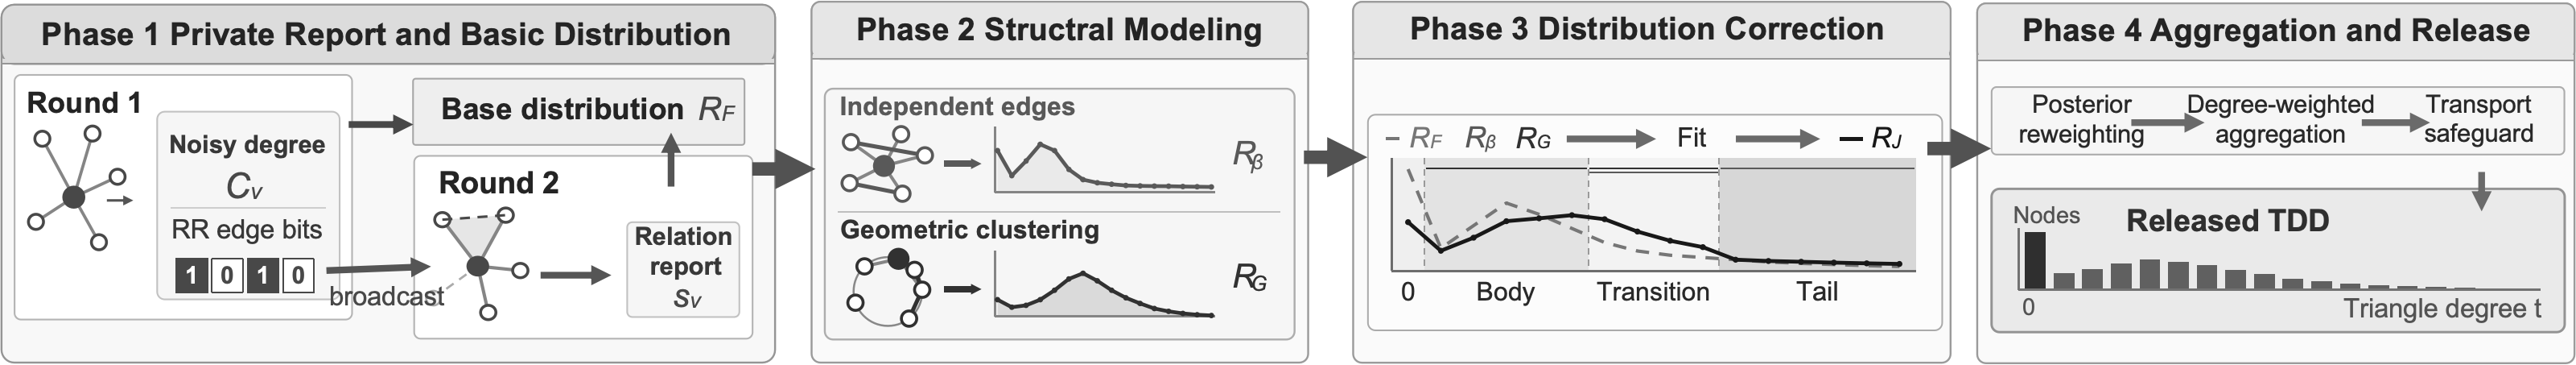
\includegraphics[width=\textwidth]{icde_sections/figures/overview.png}
  \caption{Overview of PrivTDD. }
  % Posterior aggregation forms the candidate estimate; the transport safeguard gives the released TDD.
  \label{fig:privtdd-overview}
\end{figure*}

\section{Problem}
\label{sec:problem}

\subsection{Problem Definition}
\label{subsec:problem-formulation}

% Under the graph setting in Section~\ref{sec:pre}, user $v$ holds $N_v$ and can compute $d_v,w_v$, but generally not $t_v$ because edges among its neighbors are not locally visible. An honest-but-curious server follows the protocol but may use the transcript to infer private edges. It coordinates interactions and estimates the GDD from locally randomized reports, without collecting raw adjacency lists or unperturbed degrees.
 User $v$ holds its neighborhood $N_v$ and can compute $d_v$ and $w_v$, but generally not $t_v$, because edges among its neighbors are not locally visible. An honest-but-curious server coordinates interactions and estimates the TDD from locally randomized reports, without collecting raw adjacency lists or unperturbed degrees.


% We estimate the triangle GDD $\mathbf H=(H(t))_{t\in\mathcal T}$, where $H(t)=h_G^\triangle(t)$ counts nodes participating in exactly $t$ triangles. Since $t_v\le W_{\max}=\binom{n-1}{2}$, the bin domain is $\mathcal T=\{0,\ldots,W_{\max}\}$, including zero participation and all possible counts without an overflow bin.
% \begin{definition}[LDP GDD Estimation]
% \label{def:ldp-gdd-estimation}
% Given total budget $\varepsilon$, design an interactive collection protocol $\Psi_{\mathrm{collect}}$ and server aggregation algorithm $\Phi$ to output an estimate $\widehat{\mathbf H}$ of $\mathbf H$. Local randomizers satisfy Definition~\ref{def:edge-ldp} under their allocated budgets, and the complete protocol $\Pi$ satisfies Definition~\ref{def:edge-transcript-privacy} under $\varepsilon$, protecting the presence or absence of one undirected edge. Using only privatized reports and public parameters, the output obeys $\widehat H(t)\ge0$ and $\sum_{t\in\mathcal T}\widehat H(t)=n$; estimated bin counts may be real-valued. The objective is to reduce GDD estimation error under this budget, measured by MSE, EMD, and KS in Section~\ref{sec:gdd:en:setup}.
% \end{definition}
% Each triangle contributes to three nodes, so its global count is $T_\triangle=\frac13\sum_{t\in\mathcal T}tH(t)$. Thus the GDD determines the global count, while the reverse is not true.

The target is the count histogram $\mathbf H=(H(t))_{t\in\mathcal T}$ defined in Section~\ref{sec:pre}, with $\mathcal T=\{0,\ldots,W_{\max}\}$. Here $W_{\max}=w(D_{\max})=\binom{n-1}{2}$ is the public upper bound on a node's triangle degree. Triangle degree zero is included.
\begin{definition}[Edge-LDP TDD Estimation]
\label{def:ldp-gdd-estimation}
Given total budget $\varepsilon$, design an interactive collection protocol $\Psi_{\mathrm{collect}}$ and server estimator $\Phi$ that output $\widehat{H}$. The local randomizers satisfy Definition~\ref{def:edge-ldp} under their allocated budgets, and the complete interactive protocol protects any single undirected-edge change under $\varepsilon$. Using only private reports and public parameters, the output satisfies $\widehat H(t)\ge0$ and $\sum_t\widehat H(t)=n$, with real-valued estimated bin counts allowed. We seek low histogram error, evaluated by MSE, EMD, and KS in Section~\ref{sec:gdd:en:setup}.
\end{definition}
Each triangle contributes to three nodes, so $T_\triangle=\frac13\sum_t tH(t)$. Thus the TDD determines the global triangle count, but the converse does not hold.


\subsection{Baseline Composed by Existing Operators}
\label{subsec:direct-composition}
Standard LDP frequency estimators assume that users know their contributed categories~\cite{LDPGDDWang2017,kairouz2016discrete,bassily2015succinct}, but the category $t_v$ is not locally known here. 
This composed baseline first estimates each node's triangle degree $\widetilde t_v$ using a private counting procedure, then bins the estimates.
Such procedures release noisy information about edges and local statistics~\cite{he2025robust,dong2026ldpgraph}. 
For TDD estimation, the node-level target must include all triangles containing that node, not only the contributions assigned to it for deduplicated global counting.

%Standard LDP frequency oracles require users to know their contributed categories~\cite{LDPGDDWang2017}; here the category $t_v$ is not locally known. A direct alternative first obtains privatized participation estimates $\widetilde t_v$ through an interactive counting procedure $\Pi_{\mathrm{cnt}}$, then bins them. Such procedures provide perturbed auxiliary edges and collect noisy local statistics~\cite{LDPGDDImola2022Corrected}. Procedures that assign each triangle to a single node for global counting must instead target all triangles containing each node when adapted to GDD estimation: an assigned contribution cannot directly serve as $t_v$.

% For nearest-integer rounding with a fixed tie rule, define
With nearest-integer rounding and a fixed tie rule, this composed baseline outputs
\begin{equation}
\begin{aligned}
&\mathsf b_{W_{\max}}(x)=\operatorname{round}(\operatorname{clip}_{[0,W_{\max}]}(x)),\\
&\widehat H^{\mathrm{dir}}(t)=\sum_{v\in V}\mathbf1\{\mathsf b_{W_{\max}}(\widetilde t_v)=t\}.
\end{aligned}
\label{eq:direct-gdd}
\end{equation}
Here $\operatorname{clip}_{[a,b]}(x)=\min\{b,\max\{a,x\}\}$.
Each estimate contributes one node to a single bin. 
Binning is post-processing and requires no additional privacy budget.
%each privatized estimate contributes one count to its clipped and rounded bin.

\subsection{Limitations}
\label{subsec:direct-limitations}

\noindent\textbf{Estimating locally unknown triangle degrees.}
Because $t_v$ is not directly available, estimating it from sampled, filtered, or randomized relations and noisy local statistics can introduce error before binning. Let $\eta_v=\widetilde t_v-t_v$ denote this error.

\noindent\textbf{Binning distortion.}
Positive and negative errors may cancel in a global sum, but binning changes a node's assigned category whenever its estimate crosses a boundary. 
For a fixed graph,
%In global summation, positive and negative errors in $\sum_v\eta_v$ may cancel. Binning instead moves a node's count from its true bin to another whenever its estimate crosses a boundary. For a fixed graph,
\begin{equation}
\mathbb E[\widehat H^{\mathrm{dir}}(t)\mid G]
=\sum_v\Pr[\mathsf b_{W_{\max}}(t_v+\eta_v)=t\mid G].
\label{eq:expected-direct-gdd}
\end{equation}
Even unbiased node estimates need not make this equal $H(t)$: zero-mean numerical error does not ensure balanced expected mass entering and leaving each bin.


To illustrate this limitation,
consider the six-node triangular-prism example in Fig.~\ref{fig:tdd-motivation}\subref{fig:tdd-limitation}. Every node has degree $3$, wedge count $3$, and triangle degree $1$, so $H(1)=6$. Estimates $(0,0,0,2,2,2)$ stay within these capacities and preserve both the sum of triangle degrees and the global triangle count, yet empty the true bin. This example shows that total-count accuracy alone does not imply histogram accuracy, even without capacity violations.
%To illustrate the distinction between total-count and distribution accuracy, consider disjoint triangles with $n$ a positive multiple of six. Every node has $t_v=1$, so $H(1)=n$. An illustrative estimate assigning half the nodes to bin zero and half to bin two preserves the participation sum $n$ and global triangle count $n/3$, yet empties the true bin. Binning costs no additional privacy budget, but its distribution distortion cannot be judged from global counting error alone.

%%\noindent\textbf{Motivation for Distribution Estimation.}
The \textbf{difficulty} lies in converting noisy node estimates into definite bin assignments. 
Unbiasedness and total-count accuracy alone do not control the resulting histogram error.
This motivates estimating the population histogram from private reports without first choosing a single triangle degree per node.
Such estimation can also use locally observable information, such as degrees, even when triangle degrees are unknown.
We therefore consider combining this information with noisy relational evidence to develop an operator tailored to the characteristics of TDD.
% These limitations motivate using $t_v=w_v\rho_v$ to separate scale from closure. Degrees are known locally, so the server can recover the scale distribution from privatized degree reports; closure still requires inference from relational reports. Aggregating participation probabilities retains uncertainty instead of reducing each node to one bin. At the population level,
% \begin{equation}
% H(t)=n\sum_{d=0}^{D_{\max}}\pi(d)R(t\mid d).
% \label{eq:problem-conditional-factorization}
% \end{equation}
% Here $n\pi(d)$ weights the participation distribution conditional on degree $d$, retaining dependence between scale and closure. Section~\ref{sec:method} develops the recovery procedure.

%\input{icde_sections/method_reorganize.tex}
\section{Method Overview}\label{sec:method}

\subsection{Basic Idea}
A node's triangle degree is its wedge count times its closure rate.
PrivTDD estimates the wedge-count distribution and closure-rate distributions at each node degree.
Wedge counts follow from locally known degrees, so privatized degree reports suffice to estimate their distribution without first inferring triangle degrees.
Closure rates are harder to estimate because nodes generally cannot observe edges between their neighbors.
Modeling the closure-rate distribution can reduce how much must be inferred from noisy reports.
%For example, if all nodes with wedges shared the same closure rate, the server would need to estimate only that one parameter to characterize closure.

\
\subsection{Overview}
\label{sec:overview}
As illustrated in Fig.~\ref{fig:privtdd-overview}, PrivTDD consists of four phases.
In \textbf{Phase 1}, nodes report privatized degrees and randomized adjacency bits in the first round, and the server
broadcasts these bits.
 In the second round, nodes use the broadcast bits to generate private relational reports on
connections among their retained neighbors. The server estimates the node-degree distribution and a base triangle-degree distribution conditional on node degree.
In \textbf{Phase 2}, the server constructs two complementary
structural reference distributions from the private reports,
capturing degree-driven connectivity and local clustering,
respectively.
In \textbf{Phase 3}, these references guide corrections to
the base distribution, while the private reports determine
how to adjust probability mass across triangle-degree ranges
and its within-region shape.
In \textbf{Phase 4}, the server combines the corrected
distribution with each node's reports to obtain posterior
probabilities over candidate node degrees and triangle degrees.
Aggregating these probabilities within each degree and
weighting by the estimated degree proportions yields
a candidate TDD estimate. Section~\ref{sec:aggregation} gives the final release rule.


\subsection{Challenges}
\label{sec:method_challenges}
\label{subsec:idea-challenges}
\noindent\textbf{Challenge 1. Constructing informative structural references from limited private reports.}
In Phase 2, the server must use private reports alone to construct reference distributions of triangle degrees at each node degree.
Degree $d$ fixes the number of neighbor pairs, $w(d)=\binom d2$, but reveals neither which pairs are connected nor how often their closures occur together~\cite{newman2009clustering}.
Relational reports give noisy evidence about these connections.
Even an accurate mean closure rate would leave the spread of triangle degrees undetermined.

To illustrate, fix the model parameters and the identities $\mathcal I$ of the central node and its neighbors.
For each neighbor pair $e$, let $X_e$ indicate whether it is connected and set $p_e=\Pr(X_e=1\mid\mathcal I)$.
The central node's triangle degree $T=\sum_{e=1}^{w(d)}X_e$ has conditional variance:
\begin{equation}
\begin{aligned}
\operatorname{Var}(T\mid\mathcal I)
=\sum_e p_e(1-p_e)+2\sum_{e<f}\operatorname{Cov}(X_e,X_f\mid\mathcal I).
\end{aligned}
\label{eq:challenge_closure_dependence}
\end{equation}
Even with every $p_e$ fixed, dependence among closures can change the variance of $T$.
Section~\ref{sec:references} constructs two references on the same fitted degree model. One assumes independent edges, and the other captures local clustering.

\noindent\textbf{Challenge 2. Adjusting the base distribution with structural references.}
In Phase 3, the server must decide how much to adjust the base distribution using the Phase 2 references.
A reference may fit some triangle-degree ranges better than others, yet the true TDD is unavailable for judging which adjustments to trust.
Using the Phase 1 reporting model, the server assesses how well each candidate adjustment explains the observed private reports.
Randomization limits which differences the reports can distinguish.
A single parameter ties adjustments across all count ranges together.
At the other extreme, fitting a separate unrestricted distribution at each degree requires $\sum_{d=0}^{D_{\max}}w(d)=\binom{D_{\max}+1}{3}$ free parameters in total.
Even within one range, two distinct adjustments may be needed.
For example, a reference may match the relative frequencies of tail counts while assigning too much probability to the tail.
The server must therefore adjust regional mass and within-region shape separately while keeping the distribution valid.
Section~\ref{sec:correction} fits a small set of parameters shared across degrees to the observed private reports to determine how much of each adjustment to apply.

\section{PrivTDD Detail}

\subsection{Phase 1: Private Reports and Base Distribution}
\label{sec:base}
\label{sec:private_collection}
\label{sec:distribution_construction}
Structural references and subsequent distribution correction require private evidence about node degrees and connections among neighbors.
In this Phase, we collect this evidence through a two-round reporting protocol and construct the base triangle-degree distribution.

\subsubsection{Private report collection}
The estimator uses degree reports $C_v$ and relational reports $s_v$, collected in two rounds, as $\mathcal Z=\{(C_v,s_v)\}_{v\in V}$, using positive budgets $\varepsilon_{\mathrm{deg}},\varepsilon_{\mathrm{rr}},\varepsilon_{\mathrm{rel}}$ for degree, randomized response (RR)~\cite{LDPGDDWarner1965}, and relational reporting, respectively.
In Round 1, nodes draw independent degree noise, and node $v$ releases
\begin{equation}
C_v=\operatorname{clip}_{[0,D_{\max}]}\!\left(\lfloor d_v+\xi_v\rfloor\right),
\quad \xi_v\sim\operatorname{Lap}(0,1/\varepsilon_{\mathrm{deg}}).
\label{eq:private_degree}
\end{equation}
For every unordered node pair $\{u,w\}$, one publicly assigned endpoint releases the RR version $\widetilde A_{uw}$ of its adjacency bit $x_{uw}$, independently across pairs. The server broadcasts these reports for reuse without neighborhood-dependent queries~\cite{imola2021locally}. 
We use $p,p_0$ to denote the probabilities of preserving
and flipping a bit, and set $\gamma=p-p_0$.

In Round 2, node $v$ applies neighborhood truncation with size cap $C_v$: it retains its first $\min(d_v,C_v)$ neighbors under a fixed, graph-independent public order, forming $N_v^C$. It computes the retained wedge count $\widetilde W_v$ and the count $B_v$ of RR ones, then releases only $s_v$:
\begin{equation}
\begin{alignedat}{2}
&\widetilde W_v=\binom{|N_v^C|}{2}, &\quad& B_v=\sum_{\{u,w\}\subseteq N_v^C}\widetilde A_{uw},\\
&s_v=\frac{B_v-p_0\widetilde W_v+\zeta_v}{\gamma}, &\quad& b_v=\frac{(C_v-1)_+}{\varepsilon_{\mathrm{rel}}}.
\end{alignedat}
\label{eq:private_relational_statistic}
\end{equation}
Here $(x)_+=\max\{x,0\}$. For $C_v>1$, $\zeta_v\sim\operatorname{Lap}(0,b_v)$ is independent noise; otherwise $s_v=\zeta_v=0$. The neighborhood, $\widetilde W_v$, and $B_v$ remain local. Averaging over RR and count noise gives $\mathbb E[s_v\mid N_v^C]=t_v^C$, the number of triangles containing $v$ and two nodes in $N_v^C$. It need not equal $t_v$ because $C_v<d_v$ truncates the neighborhood. Given the first-round transcript, the centered count $B_v-p_0\widetilde W_v$ has sensitivity at most $(C_v-1)_+$. Accounting for both endpoints gives
\begin{equation}
2\varepsilon_{\mathrm{deg}}+\varepsilon_{\mathrm{rr}}+
2\varepsilon_{\mathrm{rel}}\le\varepsilon.
\label{eq:privacy_allocation}
\end{equation}
The privacy proof and the budget-selection rule are in Section~\ref{sec:analysis}. Subsequent estimation uses these reports without further privacy expenditure.

\subsubsection{Scale and closure distribution estimation}
\emph{Wedge-count distribution.} Let $\mathcal K_{\mathrm{deg}}(c\mid d)=\Pr(C_v=c\mid d_v=d)$ be the channel induced by~\eqref{eq:private_degree}, including flooring and clipping, and $\mathcal P_m$ the $m$-coordinate probability simplex. Fit the population degree proportions~\cite{koenker2014convex} and assign probabilities to candidate degrees for each report:
\begin{equation}
\begin{aligned}
&\widehat\pi\in\arg\min_{\pi\in\mathcal P_{D_{\max}+1}}
-\sum_v\log\sum_{d=0}^{D_{\max}}\pi(d)\mathcal K_{\mathrm{deg}}(C_v\mid d),\\
&q_v(d)=\frac{\widehat\pi(d)\mathcal K_{\mathrm{deg}}(C_v\mid d)}
{\sum_{d'}\widehat\pi(d')\mathcal K_{\mathrm{deg}}(C_v\mid d')}.
\end{aligned}
\label{eq:degree_distribution}
% Equation label merged: eq:degree_posterior -> eq:degree_distribution
\end{equation}
The wedge-count distribution places each estimated degree probability at $w(d)$, combining degrees $0$ and $1$ at zero. Here $q_v(d)$ is node $v$'s degree posterior based only on $C_v$. Subsequent degree sums use $\mathcal D=\{d:\widehat\pi(d)>0\}$, including $d>C_v$.

\emph{Report likelihood.} We use $\rho\in[0,1]$ as a continuous working representation of closure rate. Define the full and retained wedge capacities $w(d)=\binom d2$ and $W^C_{v,d}=\binom{\min(d,C_v)}2$, the centered report $Q_v=\gamma s_v$, and the integer-count map $\tau_d(\rho)=\operatorname{round}(w(d)\rho)$ with a fixed tie rule. The likelihood $\ell_v(d,\rho)$ models $Q_v$ given $C_v$ and candidate state $(d,\rho)$. If $C_v\le1$, take $\ell_v=1$. Otherwise, for $W^C_{v,d}\le64$, assume that, conditional on $(d,t)$, all placements of the $t=\tau_d(\rho)$ closing pairs among the $w(d)$ candidate pairs are equally likely. This working assumption gives:
\begin{equation}
\begin{aligned}
&J_v\mid d,t,C_v\sim\operatorname{Hypergeom}(w(d),t,W^C_{v,d}),\\
&B_v\mid J_v=j\overset{\mathrm d}{=}
\operatorname{Bin}(j,p)+\operatorname{Bin}(W^C_{v,d}-j,p_0),\\
&\ell_v(d,\rho)=\mathbb E_{J_v,B_v}\!\left[
\frac{e^{-|Q_v-B_v+p_0W^C_{v,d}|/b_v}}{2b_v}\right].
\end{aligned}
\label{eq:projected_closing_count}
\end{equation}
Here $J_v$ is the retained true closing-edge count; 
the hypergeometric parameters are total, closing, and retained pair counts, respectively. 
Marginalizing $J_v$ and $B_v$ propagates both relational randomization and count noise into inference. 
The binomials are independent; $J_v=t$ without truncation and $J_v=t=0$ when $w(d)=0$. 
For larger retained capacities:
\begin{equation}
\ell_v(d,\rho)\approx
f_{\mathrm{NL}}\!\left(Q_v-\gamma W^C_{v,d}\rho;
\sqrt{W^C_{v,d}pp_0},b_v\right),
\label{eq:closure_likelihood}
\end{equation}
where $f_{\mathrm{NL}}(\cdot;\sigma,b)$ is the density of independent $\mathcal N(0,\sigma^2)$ plus $\operatorname{Lap}(0,b)$ noise. This approximation replaces the retained count by $W^C_{v,d}\rho$ and omits its truncation-induced variation.

\emph{Shared fit and conditional base.} To pool closure evidence, fix $K\ge4$ components: $\nu_0=\delta_0$, $\nu_{K-1}=\delta_1$, and $\nu_k=\operatorname{Unif}[e_{k-1},e_k]$ for $1\le k\le K-2$, with fixed interval boundaries $0=e_0<\cdots<e_{K-2}=1$. Here $\delta_a$ is the point mass at $a$. With mixture weights $\theta\in\mathcal P_K$, set $\mathcal G_\theta=\sum_k\theta_k\nu_k$. Let $\overline\Lambda_{vk}$ be report $v$'s likelihood under component $k$, averaged over candidate degrees, and fit:
\begin{equation}
\begin{aligned}
&\overline\Lambda_{vk}=\sum_d q_v(d)
\int_{[0,1]}\ell_v(d,\rho)\nu_k(\mathrm d\rho),\\
&\widehat\theta\in\arg\min_{\theta\in\mathcal P_K}
-\frac1n\sum_v\log\sum_k\theta_k\overline\Lambda_{vk}.
\end{aligned}
\label{eq:shared_closure_fit}
% Equation label merged: eq:closure_grid -> eq:shared_closure_fit
\end{equation}
Shared RR makes reports dependent, so this is a composite likelihood~\cite{varin2011overview}, convex in the weights. The shared weights pool information without forcing the final conditional distributions to coincide. Combine the fitted distribution with each node's evidence:
\begin{equation}
\begin{aligned}
&r_{v,d}(\mathrm d\rho)=
\frac{q_v(d)\ell_v(d,\rho)\mathcal G_{\widehat\theta}(\mathrm d\rho)}
{\sum_k\widehat\theta_k\overline\Lambda_{vk}},\\
&\widehat P_F(\mathrm d\rho\mid d)=
\frac{\sum_v r_{v,d}(\mathrm d\rho)}{\sum_v r_{v,d}([0,1])},\\
&R_F(t\mid d)=\int_{[0,1]}\mathbf1\{t=\tau_d(\rho)\}
\widehat P_F(\mathrm d\rho\mid d).
\end{aligned}
\label{eq:joint_latent_posterior}
% Equation label merged: eq:conditional_closure -> eq:joint_latent_posterior
% Equation label merged: eq:conditional_participation -> eq:joint_latent_posterior
\end{equation}
$r_{v,d}$ is the working joint degree--closure posterior, with total mass $r_{v,d}([0,1])$ equal to the updated degree probability. Normalizing within $d$ gives the conditional closure-rate distribution $\widehat P_F$ and the conditional triangle-degree distribution $R_F$. The mapping to integer counts collects probability over closure values, rather than assigning each node to a single bin. For $d\le1$, set $\widehat P_F=\delta_0$ and $R_F(0\mid d)=1$. Relational evidence updates these conditional distributions, not the population weights $\widehat\pi$. The outputs are $\widehat\pi$, $\{q_v\}$, the report likelihood $\ell_v$, and $R_F$; $n\sum_d\widehat\pi(d)R_F(t\mid d)$ is already a base TDD estimate.


\subsection{Phase 2: Complementary Structural References}
\label{sec:references}
\label{sec:gdd_reconstruction}
To address Challenge 1, both references use a shared edge-probability model fitted from privatized degree reports. The $\beta$ reference assumes conditional edge independence; the geometric reference introduces local clustering while preserving type-pair marginal edge probabilities. Their differences therefore reflect closure assumptions rather than different degree fits.

\subsubsection{Shared edge-probability model}
Compute the posterior mean degree $\bar d_v=\sum_d d q_v(d)$. For a preset maximum of $M_{\max}$ types, partition $[0,\max_v\log(1+\bar d_v)]$ into $M_{\max}$ equal-width cells and group nodes by $\log(1+\bar d_v)$, retaining nonempty types; if all means are zero, use one type. For type $a$, define its node set $V_a$, size $n_a=|V_a|$, target mean degree $\mu_a=n_a^{-1}\sum_{v\in V_a}\bar d_v$, and edge-probability parameter $\beta_a$. With $\boldsymbol\beta=(\beta_a)_a$, $\bar\beta=n^{-1}\sum_a n_a\beta_a$, and fixed parameter bound $B_\beta>0$, fit the $\beta$ model~\cite{chatterjee2011random}:
\begin{equation}
\begin{aligned}
&\widehat{\boldsymbol\beta}\in\arg\min_{|\beta_a|\le B_\beta}\frac1n
\Bigl\{\frac12\sum_{a,b}n_a(n_b-\mathbf1\{a=b\})\\
&\quad \cdot\log(1+e^{\beta_a+\beta_b})-\sum_a n_a\mu_a\beta_a\\
&\quad +\frac12\sum_a n_a(\beta_a-\bar\beta)^2\Bigr\}.
\end{aligned}
\label{eq:structural_beta_fit}
\end{equation}
The resulting edge probability is $P_{ab}=(1+e^{-\widehat\beta_a-\widehat\beta_b})^{-1}$. The penalty and bound control parameter variation and magnitude.

\subsubsection{Independent-edge reference}
A fitted $\beta_a$ does not fix realized degree, so condition on a type-$a$ central node having exactly $d$ neighbors. Let $\mathbf z=(z_h)_h$ count neighbors by type, with $z_h$ type-$h$ neighbors drawn from $N_h^{(a)}=n_h-\mathbf1\{h=a\}$ available nodes. Both references use:
\begin{equation}
\Pr(\mathbf z\mid a,d)\propto
\mathbf1\!\left\{\sum_hz_h=d\right\}
\prod_h\binom{N_h^{(a)}}{z_h}e^{\widehat\beta_hz_h},
\label{eq:fixed_degree_composition}
\end{equation}
with $0\le z_h\le N_h^{(a)}$; the factor $e^{\widehat\beta_a d}$ cancels upon normalization. Given these neighbor-type counts, the triangle degree $T_\beta$ under independent closing edges satisfies:
\begin{equation}
\begin{aligned}
&T_\beta\mid\mathbf z\overset{\mathrm d}{=}
\sum_{h<j}\operatorname{Bin}(z_hz_j,P_{hj})\\
&\quad +\sum_h\operatorname{Bin}\!\left(\binom{z_h}{2},P_{hh}\right).
\end{aligned}
\label{eq:beta_conditional_count}
\end{equation}
Averaging this count distribution with posterior weights $\eta_a(d)$ for central types at degree $d$ yields the reference $R_\beta$:
\begin{equation}
\begin{aligned}
&\eta_a(d)=\frac{\sum_{v\in V_a}q_v(d)}{\sum_vq_v(d)},\\
&R_\beta(t\mid d)=\sum_a\eta_a(d)
\mathbb E_{\mathbf z\mid a,d}[\Pr(T_\beta=t\mid\mathbf z)].
\end{aligned}
\label{eq:beta_conditional_reference}
\end{equation}

\subsubsection{Clustering reference on the same edge model}
Independent edges do not account for the extra tendency of two neighbors to connect due to latent proximity. Inspired by hidden geometric models~\cite{serrano2008selfsimilarity}, place nodes independently and uniformly on a circle of circumference one. For shortest circular distance $\delta\in[0,1/2]$ and locality parameter $0<\kappa<1$, define the connection probability:
\begin{equation}
\begin{aligned}
&a_{ab}=\kappa P_{ab},\qquad b_{ab}=\min(P_{ab}/\kappa,1),\\
&\omega_{ab}=(b_{ab}-P_{ab})/(b_{ab}-a_{ab}),\\
&g_{ab}^{(\kappa)}(\delta)=\omega_{ab}\mathbf1\{\delta\le a_{ab}/2\}\\
&\quad+(1-\omega_{ab})\mathbf1\{\delta\le b_{ab}/2\}.
\end{aligned}
\label{eq:geometry_connection_kernel}
\end{equation}
The quantities $a_{ab},b_{ab}$ are full arc lengths, mixed with weight $\omega_{ab}$. Averaging over positions gives $\omega_{ab}a_{ab}+(1-\omega_{ab})b_{ab}=P_{ab}$. Set $g_{ab}^{(0)}=P_{ab}$ and $g_{ab}^{(1)}(\delta)=\mathbf1\{\delta\le P_{ab}/2\}$ at the endpoints. Edges incident to the central node remain independent after integrating over candidate positions, so~\eqref{eq:fixed_degree_composition} still applies. Conditional on connection to a type-$a$ central node at zero, draw neighbor positions independently, with each type-$h$ neighbor having density:
\begin{equation}
f_{ah}^{(\kappa)}(x\mid\mathrm{edge})=
\frac{g_{ah}^{(\kappa)}(\delta_{\mathrm{circ}}(x,0))}{P_{ah}},
\quad x\in[-1/2,1/2).
\label{eq:geometry_conditional_position}
\end{equation}
Here $\delta_{\mathrm{circ}}$ denotes shortest circular distance. For neighbor types $h_r$ and positions $\mathbf X=(X_r)_{r=1}^d$, sum conditionally independent closures into triangle degree $T_G$ and integrate to obtain the geometric reference $R_G$:
\begin{equation}
\begin{aligned}
&T_G\mid\mathbf z,\mathbf X
\overset{\mathrm d}{=}\sum_{r<s}\operatorname{Bernoulli}
\!\left(g_{h_rh_s}^{(\kappa)}(\delta_{\mathrm{circ}}(X_r,X_s))\right),\\
&R_G(t\mid d;\kappa)=\sum_a\eta_a(d)
\mathbb E_{\mathbf z,\mathbf X\mid a,d;\kappa}
[\Pr(T_G=t\mid\mathbf z,\mathbf X)].
\end{aligned}
\label{eq:geometry_conditional_reference}
\end{equation}
Shared positions induce dependence among closures after integration, without estimating actual node locations. At $\kappa=0$, this reduces to $R_\beta$.

\emph{Selecting $\kappa$.} Using the same truncation working model as Section~\ref{sec:base}, match the predicted report mean $\mu_G^{\mathrm{rep}}(\kappa)$ to the observed mean $\bar s$:
\begin{equation}
\begin{aligned}
&\mu_G^{\mathrm{rep}}(\kappa)=\frac1n\sum_v\sum_d
q_v(d)\frac{W^C_{v,d}}{w(d)}\mathbb E[T_G\mid d;\kappa],\\
&\widetilde\mu_G^{\mathrm{rep}}(\widehat\kappa)
=\operatorname{clip}_{I_G^{\mathrm{rep}}}(\bar s),
\qquad \bar s=\frac1n\sum_vs_v.
\end{aligned}
\label{eq:geometry_calibration}
% Equation label merged: eq:geometry_population_mean -> eq:geometry_calibration
\end{equation}
Solve for $\widehat\kappa\in[0,1]$. Zero-capacity terms are zero. Here $\widetilde\mu_G^{\mathrm{rep}}$ is the numerical approximation, and $I_G^{\mathrm{rep}}$ is the interval between its endpoint predictions at $0$ and $1$. Use a matching endpoint when the target equals its prediction, and $\widehat\kappa=0$ when the endpoint predictions coincide. Fix $R_G(t\mid d)=R_G(t\mid d;\widehat\kappa)$. Both references are computed analytically for $d\le2$ and by Monte Carlo integration otherwise. Neither is assumed correct across all triangle-degree ranges.


\subsection{Phase 3: Report-Driven Distribution Correction}
\label{sec:correction}
To address Challenge 2, we use the two structural references
to correct the data-driven base $R_F$ without treating
either as ground truth.
A reference may capture the relative frequencies within
a count range but misestimate its total probability,
so we adjust regional mass and within-region shape separately.
Since randomized reports provide limited evidence,
we fit a small set of correction strengths shared across
degrees using the report likelihood.

\subsubsection{Regional mass and shape}
Using shared boundaries $b_1\le b_2$, define four degree-specific regions $I_r(d)$, separating zero from positive counts:
\begin{equation}
\begin{aligned}
&I_0(d)=\{0\},\\
&I_1(d)=(0,b_1]\cap\{1,\ldots,w(d)\},\\
&I_2(d)=(b_1,b_2]\cap\{1,\ldots,w(d)\},\\
&I_3(d)=(b_2,w(d)]\cap\mathbb Z.
\end{aligned}
\label{eq:participation_regions}
\end{equation}
These are zero, body, transition, and tail. Choose $b_1,b_2$ at two prespecified quantile levels of the base population distribution $p_F(t)=\sum_d\widehat\pi(d)R_F(t\mid d)$ conditional on $t>0$, and keep them fixed during fitting. If positive mass is absent, set both to zero; empty regions are allowed. Different regions can then change without forcing the same adjustment elsewhere.

Within a region, a reference can have a useful relative shape but an inaccurate total probability. For source $s\in\{F,G,\beta\}$ and region $r$, define regional mass $m_{sr}(d)$ and normalized shape $h_{sr}(t\mid d)$:
\begin{equation}
\begin{aligned}
&m_{sr}(d)=\sum_{t\in I_r(d)}R_s(t\mid d),\\
&h_{sr}(t\mid d)=\frac{R_s(t\mid d)\mathbf1\{t\in I_r(d)\}}{m_{sr}(d)}.
\end{aligned}
\label{eq:regional_mass_shape}
\end{equation}
Set $h_{sr}=0$ when $m_{sr}=0$. For each positive region, choose initial within-region shape $h_{0r}$ as the first nonempty shape in the order $F,G,\beta$, or zero if none exists. Set $h_{00}(t\mid d)=\mathbf1\{t=0\}$. Transferring mass along $h_{0r}$ avoids changing shape. %at the same time.

\subsubsection{Shared correction parameters}
Suppressing $(d,t)$, define total positive mass $m_s^+=\sum_{r=1}^3m_{sr}$ and its regional proportions $\phi_{sr}=m_{sr}/m_s^+$. Set $\phi_{Fr}=0$ if $m_F^+=0$; a reference with no positive mass uses $\phi_{Fr}$. Three changes $\Delta_j(t\mid d)$ to count probabilities transfer mass between zero and positive counts and redistribute it across positive regions:
\begin{equation}
\begin{aligned}
&\Delta_1=(m_G^+-m_F^+)\left(\sum_{r=1}^3\phi_{Gr}h_{0r}-h_{00}\right),\\
&\Delta_2=m_F^+\sum_{r=1}^3(\phi_{Gr}-\phi_{Fr})h_{0r},\\
&\Delta_3=m_F^+\sum_{r=1}^3(\phi_{\beta r}-\phi_{Fr})h_{0r}.
\end{aligned}
\label{eq:structural_directions}
\end{equation}
Only $\Delta_1$ changes total positive mass. For the four within-region shape directions, we fix the assignment: geometric in the body, both in the transition, and $\beta$ in the tail.
\begin{equation}
\begin{alignedat}{2}
&\Delta_4=m_{G1}(h_{G1}-h_{01}), &\quad& \Delta_5=m_{G2}(h_{G2}-h_{02}),\\
&\Delta_6=m_{\beta2}(h_{\beta2}-h_{02}), &\quad& \Delta_7=m_{\beta3}(h_{\beta3}-h_{03}).
\end{alignedat}
\label{eq:structural_shape_directions}
\end{equation}
Each direction sums to zero; shape directions also conserve regional mass. The fixed shape allocation does not restrict the mass directions. Set $R_{\mathbf x}=R_F+\sum_{j=1}^7x_j\Delta_j$, where $\mathbf x=(x_1,\ldots,x_7)$ contains seven strengths shared across degrees. They scale changes, not mixture components, and need not sum to one.

Bounds $0\le x_j\le1$ alone do not ensure nonnegativity. For each $r=0,\ldots,3$, order the three fixed shapes as $(h_{0r},h_{Gr},h_{\beta r})$ to form $\{h_{d\ell}\}_{\ell=1}^{12}$. Expanding the displayed directions in this order gives the following representation and feasible set $\mathcal C$:
\begin{equation}
\begin{aligned}
&R_{\mathbf x}(t\mid d)=\sum_{\ell=1}^{12}
[\mathbf c_d+\mathbf B_d\mathbf x]_\ell h_{d\ell}(t),\\
&\mathcal C=\{\mathbf x\in[0,1]^7:
\mathbf c_d+\mathbf B_d\mathbf x\ge0\ \forall d\in\mathcal D\}.
\end{aligned}
\label{eq:joint_feasible_domain}
\end{equation}
Here $\mathbf c_d\in\mathbb R^{12}$ has regional blocks $(m_{Fr},0,0)$, and column $j$ of $\mathbf B_d\in\mathbb R^{12\times7}$ contains the coefficients of $\Delta_j$ in these fixed shapes. These twelve coefficients express constraints; only seven parameters are learned. The constraints and zero-sum directions preserve nonnegativity, normalization, and the degree-specific count range; $\mathbf x=0$ retains the base.

\subsubsection{Learning from the observed reports}
For $w(d)>0$, define the report likelihood $\mathcal K_v(Q_v\mid d,t)=\ell_v(d,t/w(d))$; for $w(d)=0$, set $\mathcal K_v(Q_v\mid d,0)=\ell_v(d,0)$. Keep the base fit's truncation model and degree support. With report likelihood $f_v(\mathbf x)$, fit:
\begin{equation}
\begin{aligned}
&f_v(\mathbf x)=\sum_dq_v(d)\sum_{t=0}^{w(d)}
R_{\mathbf x}(t\mid d)\mathcal K_v(Q_v\mid d,t),\\
&\mathbf x^\star\in\arg\min_{\mathbf x\in\mathcal C}
\left\{-\sum_v\log f_v(\mathbf x)+\frac12\|\mathbf x\|_2^2\right\}.
\end{aligned}
\label{eq:fusion_optimization}
\end{equation}
This composite likelihood selects corrections from reports; the penalty shrinks them toward the base. The base, references, boundaries, degree probabilities, and report likelihoods are fixed during fitting. Affine report densities and linear constraints give a convex objective on positive densities. The corrected conditional distribution is $R_J=R_{\mathbf x^\star}$.


\subsection{Phase 4: Posterior Aggregation and Final Release}
Although $R_J$ provides a shared degree-conditioned distribution, individual reports may favor different triangle-degree values. 
Phase 4 uses these reports for posterior refinement and aggregation to produce the final TDD.

\label{sec:aggregation}
Using $\pi(d)$ and $R(t\mid d)$ defined in Section~\ref{sec:pre}, the population histogram satisfies:
\begin{equation}
H(t)=n\sum_{d=0}^{D_{\max}}\pi(d)R(t\mid d).
\label{eq:problem-conditional-factorization}
\end{equation}
Conditioning on degree preserves the dependence between wedge count and closure rate. The factor $n$ returns node counts rather than normalized probabilities.

Regional correction links count probabilities through seven directions, but each report can favor individual counts differently. Freeze $R_J$ and compute joint node-degree and triangle-degree probabilities $r_v^J(d,t)$ by one posterior reweighting~\cite{efron2014two}:
\begin{equation}
r_v^J(d,t)=\frac{q_v(d)R_J(t\mid d)\mathcal K_v(Q_v\mid d,t)}
{f_v(\mathbf x^\star)}.
\label{eq:frozen_joint_posterior}
\end{equation}
To preserve the estimated degree proportions $\widehat\pi$, normalize within each degree to obtain $R^\star(t\mid d)$, then aggregate:
\begin{equation}
\begin{aligned}
&R^\star(t\mid d)=\frac{\sum_vr_v^J(d,t)}
{\sum_v\sum_{t'=0}^{w(d)}r_v^J(d,t')},\\
&\widehat H_{\mathrm{raw}}(t)=n\sum_d\widehat\pi(d)R^\star(t\mid d).
\end{aligned}
\label{eq:final_gdd}
\end{equation}
If the within-degree normalization denominator for $R^\star(t\mid d)$ is zero, set $R^\star(t\mid d)=R_J(t\mid d)$. This single update can move beyond the finite correction family, but cannot add mass where $R_J=0$. The candidate estimate $\widehat H_{\mathrm{raw}}$ has total count $n$.

For the transport safeguard, let $F_{\mathrm{dir}}$ be the empirical cumulative distribution function (CDF) of $\mathsf b_{W_{\max}}(s_v)$ over the original relational reports $s_v$, using the clipping and rounding rule in Eq.~\eqref{eq:direct-gdd}. The estimated wedge-count CDF is $F_{\mathrm{cap}}(t)=\sum_d\widehat\pi(d)\mathbf1\{w(d)\le t\}$. The reference histogram has counts $H_A(t)=n[F_A(t)-F_A(t-1)]$, where $F_A(-1)=0$ and
\begin{equation}
F_A(t)=\max\{F_{\mathrm{dir}}(t),F_{\mathrm{cap}}(t)\}.
\label{eq:pg-reference-cdf}
\end{equation}
Let $\Delta=W_1(\widehat H_{\mathrm{raw}}/n,H_A/n)$, where $W_1$ is the first Wasserstein distance with ground cost $|t-u|$ between triangle degrees. For public $\tau>0$, set $\alpha=1$ if $\Delta\le\tau D_{\max}$ and $\alpha=\tau D_{\max}/\Delta$ otherwise. PrivTDD releases:
\begin{equation}
\widehat H=\alpha\widehat H_{\mathrm{raw}}+(1-\alpha)H_A.
\label{eq:pg-guard}
\end{equation}
This post-processing uses only released reports and public parameters, so it incurs no additional privacy loss.

\section{Privacy Analysis and Budget Allocation}
\label{sec:analysis}
We first prove the privacy guarantee for the PrivTDD protocol and then derive an allocation of its reporting budgets.
% First establish privacy for the complete protocol, then derive report-budget shares from the expected error bound for the released histogram.

\subsection{Privacy}
\begin{theorem}[Privacy of the complete protocol]\label{thm:pg-private}
The complete PrivTDD transcript satisfies pure $\varepsilon$-edge privacy when
\[
  2\varepsilon_d+\varepsilon_r+2\varepsilon_\ell\leq\varepsilon.
\]
Here $\varepsilon_d=\varepsilon_{\mathrm{deg}}$, $\varepsilon_r=\varepsilon_{\mathrm{rr}}$, and $\varepsilon_\ell=\varepsilon_{\mathrm{rel}}$ are the degree, RR, and relational-report budgets in Eq.~\eqref{eq:privacy_allocation}.
\end{theorem}

\begin{proof}
Changing an undirected edge incurs $2\varepsilon_d$ for its endpoint degree reports and $\varepsilon_r$ for its assigned RR report.
Fix the graph-independent public neighbor order and the first-round transcript, including the caps and shared RR table.
For an endpoint with cap $c>1$, growth of its retained set adds at most $c-1$ centered terms of magnitude at most one.
Replacing one retained neighbor preserves the pair count, so the centered-count difference is a sum of at most $c-1$ differences between RR bits, each of magnitude at most one.
Deletion is symmetric, and the centered count $B_v-p_0\widetilde{W}_v$ is zero for $c\leq1$.
Thus the conditional sensitivity is at most $(c-1)_+$.
At Laplace scale $(c-1)_+/\varepsilon_\ell$, the second round costs at most $\varepsilon_\ell$ per endpoint.
Other nodes' conditional report laws are unchanged.
Composition gives the stated budget, and estimation and the safeguard are post-processing.
\end{proof}

\subsection{Budget Allocation}
\label{sec:analysis:allocation}
\label{sec:analysis:utility}

A practical challenge is deciding how to allocate a fixed privacy budget among PrivTDD's three reporting mechanisms before data collection.
The degree budget controls noise in $C_v$, which affects both neighbor truncation and the estimated wedge-count distribution.
The relational-report budget controls the Laplace noise added to the centered count.
The RR budget affects how well randomized adjacency bits distinguish edges from nonedges and how much that same Laplace noise is amplified during debiasing.
Theorem~\ref{thm:pg-private} limits the weighted sum of these budgets. Giving more to one report leaves less for the others, and the server lacks the true TDD needed to compare the resulting errors.
% Budgets are chosen before collection. The degree budget affects truncation and wedge counts; the relational budget controls Laplace noise.
% The RR budget affects edge distinguishability and noise amplification during debiasing. The true histogram is unavailable for choosing shares.


Our idea is to derive an upper bound on the expected EMD of the released histogram and minimize it before collection.
Let $h=H/n$, $h_A=H_A/n$, and $\widehat h=\widehat H/n$ denote the normalized true, reference, and released histograms. Thus $\operatorname{EMD}(\widehat H,H)=W_1(\widehat h,h)$.
Phase~4 forms $H_A$ from binned relational reports and estimated wedge counts. For any graph on $n$ nodes, the reporting mechanisms give an error bound for each input in terms of the candidate budgets.
The release rule in Eq.~\eqref{eq:pg-guard} keeps $W_1(\widehat h,h_A)\leq\tau D$, with $D=D_{\max}=n-1$ and fixed public $\tau>0$.
Consequently, an expected error bound $B_A$ for $h_A$ gives $B_A+\tau D$ for $\widehat h$. $B_A$ varies across allocations.
% Direct binning and wedge-count estimation contribute two reference-histogram errors; Phase 4 relates both to the released histogram.
% Histograms have total count n and are normalized only for distances. The fixed radius means allocation compares only B_A.

\begin{lemma}[Error of the reference histogram]\label{lem:pg-reference}
Suppose Phase~1 uses all retained neighbor pairs and fits the degree proportions $\widehat\pi$ by exact maximum likelihood on $\{0,\ldots,D\}$.
Let $p=e^{\varepsilon_r}/(1+e^{\varepsilon_r})$ and $p_0=1-p$ be the RR probabilities of reporting one for an edge and a nonedge, as in Section~\ref{sec:private_collection}. Set $\gamma=p-p_0$ and $W_{\max}=\binom D2$.
Averaging over protocol randomness for any fixed $G$ gives $\mathbb E_G W_1(h_A,h)\leq B_A$, where
\begin{equation}
\begin{aligned}
B_A={}&\frac{\sqrt{pp_0 W_{\max}}}{\gamma}
       +\frac{D-1}{\gamma\varepsilon_\ell}
       +\frac{D-1}{2(1-e^{-\varepsilon_d})}+\frac12\\
     &+(D-1)\bigl[\coth(\varepsilon_d/2)+1/\varepsilon_d+1\bigr].
\end{aligned}
\label{eq:pg-anchor-bound}
\end{equation}
\end{lemma}
% This bound assumes full reporting and exact full-degree-domain maximum likelihood. The first line accounts for RR noise, Laplace noise, truncation, and rounding; the second accounts for wedge-count error.
\begin{proof}
Pair each binned relational report with its true triangle degree $t_v$. Given $C_v$ and the fixed graph, the RR count has standard deviation at most $\sqrt{pp_0W_{\max}}$ and the expected absolute Laplace noise is at most $(D-1)/\varepsilon_\ell$. Debiasing divides both by $\gamma$.
Each omitted neighbor costs at most $D-1$ triangles. With $a=\varepsilon_d$, Eq.~\eqref{eq:private_degree} gives $\mathbb E_G(d_v-C_v)_+=\tfrac12\sum_{k=0}^{d_v-1}e^{-ak}\leq[2(1-e^{-a})]^{-1}$.
Clipping cannot increase error and rounding adds at most $1/2$. This nodewise coupling allows shared RR bits.
% Pair each report with its true triangle degree to accumulate error; independence across nodes' RR reports is not required.

For the wedge counts, write $K=\mathcal K_{\mathrm{deg}}$ for the degree-report channel in Eq.~\eqref{eq:degree_distribution}. Set $f(c)=\sum_d\widehat\pi(d)K(c\mid d)$ and $g_j=n^{-1}\sum_v K(C_v\mid j)/f(C_v)$.
At the maximum, the log-likelihood derivative toward unit mass at $j$ is $n(g_j-1)\leq0$. Since $\sum_j\widehat\pi(j)g_j=1$, the mean degree posterior is $\bar q(d):=n^{-1}\sum_v q_v(d)=\widehat\pi(d)g_d=\widehat\pi(d)$.
For the floored and clipped Laplace channel,
\[
 |d-c|K(c\mid d)\leq\sum_{j=0}^D e^{-a|j-d|}K(c\mid j).
\]
For each integer $j$ from $d$ toward $c$, excluding $c$, the Laplace channel gives $K(c\mid j)=e^{a|j-d|}K(c\mid d)$.
Set $c=C_v$, multiply by $\widehat\pi(d)/(n f(C_v))$, and sum over $v,d$.
Using $g_j\leq1$ gives $n^{-1}\sum_{v,d}q_v(d)|d-C_v|\leq\sum_{k\in\mathbb Z} e^{-a|k|}=\coth(a/2)$.
Coupling each cap to its true degree adds expected cost at most $1/a+1$. The map $w(d)=\binom d2$ is $(D-1)$-Lipschitz, giving the last term of $B_A$.
% Full-domain first-order conditions equate the mean degree posterior and fitted degree law. Two couplings bound posterior-to-cap and cap-to-true-degree distances.
% The wedge-count map amplifies this distance by at most D-1.

Let $F_G$ and $F_{\mathrm{cap},G}$ be the true triangle-degree and wedge-count CDFs. Since $t_v\leq w(d_v)$, we have $F_G\geq F_{\mathrm{cap},G}$ pointwise.
The maximum in Eq.~\eqref{eq:pg-reference-cdf} gives
$|F_A-F_G|\leq|F_{\mathrm{dir}}-F_G|+|F_{\mathrm{cap}}-F_{\mathrm{cap},G}|$.
Integrating proves the claim~\cite{vallender1974distance}.
\end{proof}

\begin{theorem}[Minimax EMD for TDD]\label{thm:pg-risk}
Under the assumptions of Lemma~\ref{lem:pg-reference}, the first inequality holds for every feasible positive budget allocation. The second line gives the minimax order for fixed $\varepsilon>0$.
\begin{equation}
\begin{aligned}
 \sup_G\mathbb E_G\operatorname{EMD}(\widehat H,H)
     &\leq B_A+\tau D,\\
 \inf_\Pi\sup_G\mathbb E_G\operatorname{EMD}(\Pi(G),H)
     &=\Theta_{\varepsilon}(n).
\end{aligned}
\label{eq:pg-minimax}
\end{equation}
Here $G$ ranges over simple graphs on the public vertex set and $\Pi$ over local protocols with the same edge privacy budget that release a histogram $\Pi(G)$ of total count $n$.
For fixed $\varepsilon,\tau>0$ and budget shares bounded away from 0, $B_A+\tau D=O(n)$. Unnormalized transport cost is $n\operatorname{EMD}$ with minimax order $\Theta_\varepsilon(n^2)$.
\end{theorem}
% The finite-sample upper bound holds for every feasible positive split; the lower bound gives worst-case growth in n at fixed total budget.
\begin{proof}
By the mixture in Eq.~\eqref{eq:pg-guard}, the one-dimensional CDF formula gives $W_1(\widehat h,h_A)=\alpha\Delta\leq\tau D$. The triangle inequality and Lemma~\ref{lem:pg-reference} give the upper bound. For the lower bound, set $m=\lfloor(n-2)/4\rfloor$ for $n\geq6$ and form a clique on $2m+2$ vertices. Join each new vertex pair $i$, $1\leq i\leq m$, to the first $2i$ clique vertices. An independent fair bit $X_i$ determines the edge within pair $i$. Leave the remaining vertices isolated.
Each vertex of pair $i$ has triangle degree $a_i=\binom{2i}{2}$ or $a_i+2i$. The intervals $[a_i,a_i+2i)$ are disjoint and all clique vertices have at least $a_m+2m$ triangles.
At each of the $2i$ integer cutoffs in interval $i$, the cumulative count therefore takes two values differing by two according to $X_i$.
Edge privacy bounds the posterior odds of $X_i$ given the transcript between $e^{-\varepsilon}$ and $e^\varepsilon$, giving expected absolute count error at least $2/(1+e^\varepsilon)$ per cutoff.
Summing over cutoffs and dividing by $n$ gives average risk at least $2m(m+1)/[n(1+e^\varepsilon)]=\Omega_\varepsilon(n)$. Worst-case risk is at least as large.
\end{proof}

\emph{Approximate degree fits.}
For an approximate fit, let $r_{\mathrm{opt}}=\max_{0\leq j\leq D}g_j-1$ with the scores defined above.
The total variation distance between $\bar q$ and $\widehat\pi$ is at most $r_{\mathrm{opt}}$ since $\bar q(d)=\widehat\pi(d)g_d$. The posterior-to-cap coupling now costs at most $(1+r_{\mathrm{opt}})\coth(\varepsilon_d/2)$.
Thus the upper bound increases by at most $(D-1)[D+\coth(\varepsilon_d/2)]\mathbb E_G r_{\mathrm{opt}}$, using degree-domain diameter $D$.
For fixed $\varepsilon,\tau>0$ and budget shares bounded away from zero, the $O(n)$ rate holds if $\sup_G\mathbb E_G r_{\mathrm{opt}}=O(1/D)$. Even for a restricted grid, this residual uses scores at every degree.
% Restricted-grid or early-stopped fits require a full-domain residual check. The allocation below optimizes the public exact-fit bound before collection.

\noindent\textbf{Allocation scheme.}
We choose the budgets using the explicit full-domain, exact-fit bound $B_A+\tau D$ in Eq.~\eqref{eq:pg-minimax}. Its dependence on each budget distinguishes splits with the same $O(n)$ rate.
With the radius fixed, $B_A$ decreases in each of the three budgets. The minimizing split therefore exhausts the budget.
Writing $x=\varepsilon_d$ and $y=\varepsilon_r$ gives $\varepsilon_\ell=(\varepsilon-2x-y)/2$.
% Fix public inputs before collection and exhaust the privacy budget. Eliminating the relational-report budget leaves two optimization variables.

\begin{proposition}[Bound-optimal allocation]\label{prop:pg-allocation}
The allocation minimizing $B_A+\tau D$ is determined by the unique solution $(x^\star,y^\star)$ of
\begin{equation}
\begin{aligned}
\min_{\substack{x,y>0\\2x+y<\varepsilon}}\quad
 &\frac{\sqrt{D/[2(D-1)]}}{2\sinh(y/2)}
  +\frac{2\coth(y/2)}{\varepsilon-2x-y}\\[-1pt]
 &{}+\frac54\coth(x/2)+\frac1x .
\end{aligned}
\label{eq:pg-allocation}
\end{equation}
\end{proposition}
\begin{proof}
Substituting $\gamma=\tanh(y/2)$ and $\varepsilon_\ell=(\varepsilon-2x-y)/2$ into $B_A+\tau D$, removing constants, and dividing by $D-1$ gives Eq.~\eqref{eq:pg-allocation}.
The first and last terms are strictly convex in $y$ and $x$, respectively. The third term is convex.
The second term is log-convex because $[\log\coth(y/2)]''=\cosh(y)/\sinh^2(y)>0$ and $-\log(\varepsilon-2x-y)$ is convex.
Strict convexity and divergence at the boundary of the  domain give a unique interior minimizer. Its upper bound is at most that of the feasible split $\varepsilon_d=\varepsilon_r=\varepsilon_\ell=\varepsilon/5$, hence is $O(n)$ for fixed $\varepsilon,\tau$.
\end{proof}
Before Round~1, numerically minimize the two-variable objective in Eq.~\eqref{eq:pg-allocation} using only the public $n$ and $\varepsilon$.
Use $\varepsilon_d=x^\star$ per degree report, $\varepsilon_r=y^\star$ per assigned RR report, and $\varepsilon_\ell=(\varepsilon-2x^\star-y^\star)/2$ per relational report.
% The optimal bound is no larger than for epsilon/5 per mechanism and therefore attains the established minimax order.
% Fix all budgets before Round 1. Both endpoints consume degree and relational budgets; each edge has one RR report from its assigned endpoint.

\providecommand{\gddset}[2]{\expandafter\gdef\csname gddvalue@#1\endcsname{#2}}
\providecommand{\gddmissing}{\textcolor{blue}{\ensuremath{[\,\cdots\,]}}}
\providecommand{\gddresult}[1]{%
  \ifcsname gddvalue@#1\endcsname
    \expandafter\ifx\csname gddvalue@#1\endcsname\empty
      \gddmissing
    \else\csname gddvalue@#1\endcsname\fi
  \else\gddmissing\fi}
\providecommand{\gddci}[3]{\shortstack{\ensuremath{#1}\\[-1pt]{\scriptsize\ensuremath{[#2,#3]}}}}
\providecommand{\gddvaluesfile}{experiment_values.tex}
\InputIfFileExists{\gddvaluesfile}{}{}
\providecommand{\gddfigdir}{icde_sections/figures}
\providecommand{\gddimage}[3]{%
  \IfFileExists{\gddfigdir/#1.pdf}{%
    \includegraphics[width=\linewidth]{\gddfigdir/#1.pdf}%
  }{\IfFileExists{\gddfigdir/#1.png}{%
    \includegraphics[width=\linewidth]{\gddfigdir/#1.png}%
  }{%
    \fbox{\begin{minipage}[c][#2][c]{\dimexpr\linewidth-2\fboxsep-2\fboxrule\relax}
      \centering\small\sffamily #3\par\medskip
      \texttt{\detokenize{#1.pdf}}
    \end{minipage}}%
  }}%
}

% Reviewed experiment revision: RQ1--RQ4 and E1--E4 are retained.
% Enter dataset statistics, numerical results, and interpretation fields in icde_sections/experiment_values.tex.
% Figure filenames and cross-reference labels are defined in icde_sections/figures/.
% Empty result fields render as blue xxx; no empirical conclusion is prefilled.
\section{Experiments}\label{sec:gdd:en}
We evaluate PrivTDD's estimation accuracy, the contributions of its designs, sensitivity to the choice of regions, and the effect of sampling on TDD estimation error.
% We evaluate PrivTDD's estimation of the triangle-participation distribution through four research questions:
% \textbf{RQ1:} How accurately does PrivTDD estimate the distribution compared with existing methods?
% \textbf{RQ2:} How do structural modeling and learning correction strengths from private reports affect estimation?
% \textbf{RQ3:} How sensitive is PrivTDD to the choice of regions?
% \textbf{RQ4:} How does neighbor-pair sampling affect TDD estimation error on large networks?

\subsection{Experimental Setup}\label{sec:gdd:en:setup}

\noindent\textbf{Datasets.}
We use four real networks from SNAP and Network Repository~\cite{snapnets,rossi2015networkrepository}: the protein interaction network Bio-DMELA~\cite{singh2008alignment} with \gddresult{data.biodmela.n} nodes and \gddresult{data.biodmela.m} edges; 
the scientific collaboration network DBLP~\cite{yang2012communities} with \gddresult{data.dblp.n} nodes and \gddresult{data.dblp.m} edges; 
the social network Higgs social~\cite{dedomenico2013rumor} with \gddresult{data.higgs.n} nodes and \gddresult{data.higgs.m} edges; 
and Orkut~\cite{mislove2007measurement} with \gddresult{data.orkut.n} nodes and \gddresult{data.orkut.m} edges.
These networks cover different sizes, clustering levels, and TDDs.
We convert all inputs to simple undirected graphs, remove self-loops and duplicate edges, and retain all explicitly declared nodes and connected components; sizes refer to preprocessed graphs.

\noindent\textbf{Baselines.}
We compare PrivTDD with methods based on node-level counting and graph synthesis.
\textbf{TriTR-Hist} adapts TriTR~\cite{guo2026tritr}, 
a two-round triangle-counting estimator that Guo et al.\ identify as equivalent to TDP-VC~\cite{he2025robust}.
We adjust each node's estimate to count each incident triangle once, then clip, round, and bin the estimates.
%\textbf{TriTR-Hist}~\cite{guo2026tritr,he2025robust} converts TriTR's node triangle-participation estimates into a histogram, correcting counting multiplicities and applying clipping and rounding before binning~\cite{guo2026tritr}.
For LDPGraph~\cite{dong2026ldpgraph}, \textbf{LDPGraph-T} bins consistency-corrected node triangle-degree estimates, whereas \textbf{LDPGraph-S} recomputes the histogram on the final synthetic graph.
The outputs share private reports, isolating the effect of graph synthesis on TDD estimation.
Baselines follow their original parameter settings, adapted to the privacy-accounting convention used in this paper.

\begin{table*}[!t]
\centering
\caption{Estimation error on four networks across eight privacy budget settings}
\label{tab:gdd:e1:accuracy}
% One shade setting for all PrivTDD values. Larger numbers are lighter.
\newcommand*{\EOnePrivShade}{\cellcolor[gray]{0.90}}
\fontsize{8.5}{10}\selectfont
\setlength{\tabcolsep}{2.4pt}
\renewcommand{\arraystretch}{1.08}
\begin{tabularx}{\linewidth}{@{}lc *{12}{>{\raggedleft\arraybackslash}X}@{}}
\toprule
 &  & \multicolumn{3}{c}{PrivTDD (Ours)} & \multicolumn{3}{c}{TriTR-Hist} & \multicolumn{3}{c}{LDPGraph-T} & \multicolumn{3}{c}{LDPGraph-S} \\
\cmidrule(lr){3-5}\cmidrule(lr){6-8}\cmidrule(lr){9-11}\cmidrule(l){12-14}
Datasets & $\varepsilon$ & $10^3$\,MSE & EMD & $100$\,KS & $10^3$\,MSE & EMD & $100$\,KS & $10^3$\,MSE & EMD & $100$\,KS & $10^3$\,MSE & EMD & $100$\,KS \\
\midrule
\multirow{8}{*}{Bio-DMELA} & 0.5 & \EOnePrivShade 350.64 & \EOnePrivShade \textbf{20.39} & \EOnePrivShade \textbf{31.61} & 226.51 & 22145.74 & 49.98 & \textbf{221.81} & 965.06 & 45.60 & 615.10 & 739.05 & 57.95 \\
 & 1 & \EOnePrivShade \textbf{137.72} & \EOnePrivShade \textbf{5.05} & \EOnePrivShade \textbf{20.10} & 226.57 & 5406.54 & 49.70 & 215.78 & 175.16 & 41.51 & 505.46 & 149.62 & 50.06 \\
 & 1.5 & \EOnePrivShade \textbf{65.16} & \EOnePrivShade \textbf{2.89} & \EOnePrivShade \textbf{14.50} & 226.55 & 2453.85 & 49.38 & 205.95 & 68.61 & 37.96 & 447.99 & 61.65 & 46.75 \\
 & 2 & \EOnePrivShade \textbf{50.74} & \EOnePrivShade \textbf{2.03} & \EOnePrivShade \textbf{12.69} & 226.63 & 1425.10 & 49.02 & 193.47 & 36.39 & 35.05 & 409.87 & 33.96 & 44.45 \\
 & 2.5 & \EOnePrivShade \textbf{38.22} & \EOnePrivShade \textbf{1.58} & \EOnePrivShade \textbf{10.79} & 226.49 & 945.43 & 48.67 & 179.42 & 22.35 & 32.25 & 379.08 & 21.62 & 42.50 \\
 & 3 & \EOnePrivShade \textbf{21.24} & \EOnePrivShade \textbf{1.22} & \EOnePrivShade \textbf{8.05} & 226.44 & 681.66 & 48.34 & 164.62 & 15.19 & 30.03 & 347.25 & 15.30 & 40.47 \\
 & 3.5 & \EOnePrivShade \textbf{17.08} & \EOnePrivShade \textbf{1.00} & \EOnePrivShade \textbf{7.54} & 226.48 & 520.30 & 48.02 & 148.83 & 10.83 & 27.78 & 319.76 & 11.49 & 38.64 \\
 & 4 & \EOnePrivShade \textbf{12.46} & \EOnePrivShade \textbf{0.81} & \EOnePrivShade \textbf{6.42} & 226.38 & 413.88 & 47.71 & 133.93 & 8.31 & 25.64 & 293.49 & 9.28 & 36.87 \\
\midrule
\multirow{8}{*}{DBLP} & 0.5 & \EOnePrivShade \textbf{217.98} & \EOnePrivShade \textbf{9.33} & \EOnePrivShade \textbf{26.23} & 391.80 & 22090.15 & 49.08 & 386.00 & 919.83 & 35.96 & 294.10 & 887.25 & 36.21 \\
 & 1 & \EOnePrivShade \textbf{55.88} & \EOnePrivShade \textbf{4.62} & \EOnePrivShade \textbf{11.63} & 390.88 & 5382.79 & 47.97 & 369.61 & 157.12 & 34.66 & 331.00 & 153.39 & 32.99 \\
 & 1.5 & \EOnePrivShade \textbf{27.98} & \EOnePrivShade \textbf{3.59} & \EOnePrivShade \textbf{7.91} & 389.47 & 2437.97 & 46.97 & 347.42 & 57.16 & 34.15 & 318.82 & 56.63 & 33.14 \\
 & 2 & \EOnePrivShade \textbf{14.14} & \EOnePrivShade \textbf{2.65} & \EOnePrivShade \textbf{5.65} & 387.77 & 1412.67 & 46.00 & 323.21 & 28.24 & 33.37 & 298.46 & 28.51 & 32.68 \\
 & 2.5 & \EOnePrivShade \textbf{17.36} & \EOnePrivShade \textbf{2.09} & \EOnePrivShade \textbf{6.04} & 385.79 & 934.89 & 45.04 & 298.78 & 15.90 & 32.41 & 276.12 & 16.43 & 31.93 \\
 & 3 & \EOnePrivShade \textbf{12.40} & \EOnePrivShade \textbf{1.68} & \EOnePrivShade \textbf{5.75} & 383.63 & 672.32 & 44.12 & 275.68 & 10.02 & 31.30 & 255.05 & 10.88 & 31.01 \\
 & 3.5 & \EOnePrivShade \textbf{10.04} & \EOnePrivShade \textbf{1.40} & \EOnePrivShade \textbf{5.59} & 381.33 & 511.77 & 43.25 & 253.58 & 6.56 & 30.11 & 234.60 & 7.56 & 29.99 \\
 & 4 & \EOnePrivShade \textbf{10.01} & \EOnePrivShade \textbf{1.23} & \EOnePrivShade \textbf{5.69} & 378.92 & 405.98 & 42.44 & 234.47 & 4.75 & 28.91 & 216.86 & 5.75 & 28.92 \\
\midrule
\multirow{8}{*}{Higgs social} & 0.5 & \EOnePrivShade 24.55 & \EOnePrivShade \textbf{519.23} & \EOnePrivShade \textbf{14.42} & 301.41 & 26922.00 & 43.97 & 292.78 & 3845.87 & 37.15 & \textbf{7.29} & 4410.46 & 25.34 \\
 & 1 & \EOnePrivShade 29.00 & \EOnePrivShade \textbf{258.05} & \EOnePrivShade \textbf{17.44} & 292.42 & 6565.15 & 38.97 & 258.01 & 758.54 & 34.86 & \textbf{4.28} & 1969.99 & 18.80 \\
 & 1.5 & \EOnePrivShade 28.57 & \EOnePrivShade \textbf{130.81} & \EOnePrivShade 15.90 & 279.87 & 2904.04 & 36.22 & 212.93 & 261.19 & 31.63 & \textbf{3.32} & 1368.33 & \textbf{15.02} \\
 & 2 & \EOnePrivShade 27.28 & \EOnePrivShade \textbf{73.65} & \EOnePrivShade 13.03 & 265.88 & 1629.65 & 35.26 & 169.21 & 113.32 & 28.15 & \textbf{2.97} & 1092.75 & \textbf{12.71} \\
 & 2.5 & \EOnePrivShade 8.86 & \EOnePrivShade \textbf{45.52} & \EOnePrivShade 10.85 & 251.72 & 1042.36 & 34.25 & 132.34 & 57.61 & 24.86 & \textbf{2.72} & 1014.82 & \textbf{10.58} \\
 & 3 & \EOnePrivShade 4.79 & \EOnePrivShade \textbf{31.40} & \EOnePrivShade \textbf{9.10} & 237.95 & 725.90 & 33.24 & 102.75 & 33.06 & 21.86 & \textbf{2.59} & 984.85 & 9.24 \\
 & 3.5 & \EOnePrivShade 3.46 & \EOnePrivShade 23.32 & \EOnePrivShade \textbf{7.88} & 224.96 & 536.52 & 32.27 & 79.57 & \textbf{20.34} & 19.20 & \textbf{2.45} & 967.49 & 8.17 \\
 & 4 & \EOnePrivShade 2.66 & \EOnePrivShade 18.27 & \EOnePrivShade \textbf{6.98} & 213.04 & 414.59 & 31.35 & 62.90 & \textbf{14.00} & 17.03 & \textbf{2.40} & 962.87 & 7.49 \\
\midrule
\multirow{8}{*}{Orkut} & 0.5 & \EOnePrivShade \textbf{2.75} & \EOnePrivShade \textbf{182.69} & \EOnePrivShade \textbf{5.72} & 416.15 & 29051.16 & 45.25 & 402.88 & 5331.46 & 44.51 & 72.84 & 5215.75 & 27.31 \\
 & 1 & \EOnePrivShade \textbf{0.96} & \EOnePrivShade \textbf{116.53} & \EOnePrivShade \textbf{3.85} & 400.84 & 7186.61 & 44.40 & 344.76 & 1120.53 & 41.17 & 81.92 & 1123.67 & 26.80 \\
 & 1.5 & \EOnePrivShade \textbf{1.45} & \EOnePrivShade \textbf{66.66} & \EOnePrivShade \textbf{2.38} & 379.62 & 3201.31 & 43.20 & 272.57 & 418.09 & 36.60 & 86.11 & 446.54 & 25.74 \\
 & 2 & \EOnePrivShade \textbf{1.79} & \EOnePrivShade \textbf{35.58} & \EOnePrivShade \textbf{2.66} & 355.64 & 1803.13 & 41.80 & 205.70 & 197.35 & 31.78 & 90.89 & 234.14 & 24.60 \\
 & 2.5 & \EOnePrivShade \textbf{2.07} & \EOnePrivShade \textbf{21.15} & \EOnePrivShade \textbf{3.11} & 331.05 & 1154.47 & 40.31 & 152.26 & 107.46 & 27.33 & 81.16 & 148.65 & 21.97 \\
 & 3 & \EOnePrivShade \textbf{2.31} & \EOnePrivShade \textbf{15.20} & \EOnePrivShade \textbf{3.42} & 307.18 & 802.00 & 38.81 & 111.84 & 63.87 & 23.40 & 64.75 & 100.83 & 19.06 \\
 & 3.5 & \EOnePrivShade \textbf{2.37} & \EOnePrivShade \textbf{12.50} & \EOnePrivShade \textbf{3.59} & 284.79 & 589.83 & 37.35 & 82.25 & 40.34 & 20.05 & 48.92 & 76.07 & 16.31 \\
 & 4 & \EOnePrivShade \textbf{2.38} & \EOnePrivShade \textbf{11.00} & \EOnePrivShade \textbf{3.63} & 264.09 & 452.55 & 35.95 & 61.89 & 27.75 & 17.38 & 36.87 & 64.45 & 13.99 \\
\bottomrule
\end{tabularx}
\par\vspace{3pt}
\begin{minipage}{\linewidth}\fontsize{8}{9.3}\selectfont\raggedright Bold marks the lowest mean for each dataset, budget, and metric.
\end{minipage}
\end{table*}


\noindent\textbf{Metrics.}
We report mean squared error (MSE), earth mover's distance (EMD), and Kolmogorov--Smirnov distance (KS); lower is better.
Let $H$ and $\widehat H$ be the true and estimated node-count histograms, and let $F(t)=n^{-1}\sum_{u=0}^{t}H(u)$ be the true cumulative distribution, with $\widehat F$ defined analogously.
The metrics are
\begin{equation}
\begin{aligned}
&\mathrm{MSE}=\frac{\|\widehat H-H\|_2^2}{W_{\max}+1},\mathrm{EMD}=\|\widehat F-F\|_1,\\
&\mathrm{KS}=\|\widehat F-F\|_\infty,
\end{aligned}
\label{eq:gdd:en:metrics}
\end{equation}
where $W_{\max}=\binom{n-1}{2}$ and norms are evaluated on the integer triangle-degree domain $0,\ldots,W_{\max}$.
MSE compares node frequencies at each count; EMD accounts for both the probability mass displaced and its distance~\cite{rubner2000emd}; KS captures the largest cumulative-proportion discrepancy.
For PrivTDD, $\widehat H$ in these metrics is the released TDD in Eq.~\eqref{eq:pg-guard}.

\noindent\textbf{Implementation.}
We ran PrivTDD with \gddresult{hardware.software} on an \gddresult{hardware.processor} with \gddresult{hardware.memory.gib} GiB of memory.
For each network and privacy budget, we used the allocation in Eq.~\eqref{eq:pg-allocation} and set $\tau=1$.
By default, we use $K=\gddresult{settings.closure_components}$ closure-mixture components.
Following Section~\ref{sec:correction}, we define the body, transition, and tail regions using quantile levels $(\gddresult{settings.region_quantiles})$ of the base population distribution conditional on positive triangle degrees.
Complete parameters, baseline adaptations, and reproduction scripts are provided in the accompanying artifact.
%\footnote{Artifact: \gddresult{artifact.link}\label{fn:gdd:artifact}}
%todo in abstract+intro
% Budget optimality refers to the theoretical bound for the final safeguarded release.
% Budget optimality concerns the theoretical bound for the final release; the artifact supplies detailed implementation settings.
For E1 and E2, we scheduled \gddresult{runs.main.small_graphs} independent runs per setting on Bio-DMELA and DBLP and \gddresult{runs.main.large_graphs} on Higgs social and Orkut. We report means over completed runs and pointwise 95\% bootstrap confidence intervals.
Ablation variants share the private reports from each run.
For E4, we sampled candidate neighbor pairs after projection on Higgs social and Orkut at $\varepsilon=2$, using the same five seeds at each of the four sampling rates. Each run estimated the TDD of the full network.
% E4 fixes epsilon=2 on Higgs social and Orkut and samples projected candidate neighbor pairs. All four rates use the same five seeds and estimate the original graph TDD.
More details and results are available in the Supplementary Material. %give the full E1 intervals and paired E2 comparisons.
% E1/E2 plan 20 repetitions on each small graph and 10 on each large graph. Means and pointwise 95% bootstrap intervals use completed runs; E2 pairs the same private reports.

\subsection{Overall Estimation Accuracy (E1)}\label{sec:gdd:en:accuracy}
Table~\ref{tab:gdd:e1:accuracy} compares PrivTDD (shaded in gray) with TriTR-Hist, LDPGraph-T, and LDPGraph-S at eight total privacy budgets from $\varepsilon=0.5$ to $4$. %The means use 1,916 of 1,920 planned releases.
Across the four networks, PrivTDD had the lowest mean EMD in 30 of 32 network--budget settings, the lowest mean KS in 29, and the lowest mean MSE in 23.
Mean EMD decreased at every successive budget for PrivTDD on all four networks. MSE and KS varied less regularly. On Orkut, their minima occurred at $\varepsilon=1$ and $1.5$, respectively.
On DBLP at $\varepsilon=2$, the mean EMD of PrivTDD was 2.65 (95\% CI $[2.59,2.71]$), 90.6\% lower than the best baseline, LDPGraph-T (28.24).

PrivTDD ranked first on all three metrics at every budget on DBLP and Orkut. On Bio-DMELA, the single exception was MSE at $\varepsilon=0.5$, where LDPGraph-T had the lowest mean.
LDPGraph-S attained the lowest MSE at all eight budgets on Higgs social and the lowest KS at $\varepsilon\in\{1.5,2,2.5\}$. LDPGraph-T had the lowest EMD there at $\varepsilon\in\{3.5,4\}$.
Using only run indices completed by all four methods gave the same rankings in both settings with convergence failures.
To isolate the effect of synthesis, we compared the LDPGraph-T histogram with the histogram of the synthetic graph from the same private reports.
On the original metric scales, synthesis on Higgs social at $\varepsilon=2$ reduced MSE by 0.1662 and KS by 0.1544, while EMD rose by 979.4 (paired 95\% CI $[969.5,990.3]$).
On this network, synthesis reduced the bin-frequency error and the maximum CDF discrepancy but increased how far probability mass was displaced.


\subsection{Effects of the Core Designs (E2)}\label{sec:gdd:en:ablation}
PrivTDD, SCRec, and the three fixed-strength variants share the private reports, base fit, posterior reweighting, aggregation, and transport safeguard.
%Of 480 planned releases, 476 yielded all five outputs.
Two PrivTDD fits failed to converge on Higgs social at $\varepsilon=0.5$ and two on Orkut at $\varepsilon=4$, leaving eight matched runs in each setting.
% All five outputs share reports, base recovery, the final posterior update, aggregation, and transport safeguard. Of 480 planned conditions, 476 have complete five-method pairs; Higgs at 0.5 and Orkut at 4 each have two unconverged Full runs.

% Select one E2 figure layout.
% Four individual network plots share a single-column float, one legend and one caption.
\begin{figure}[tbhp]
\centering

\includegraphics[width=\columnwidth]{icde_sections/figures/gdd_ablation_key.pdf}\par
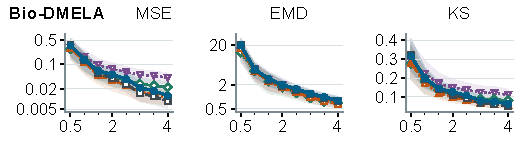
\includegraphics[width=\columnwidth]{icde_sections/figures/gdd_ablation_bio_dmela.pdf}\par
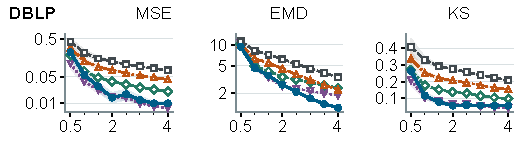
\includegraphics[width=\columnwidth]{icde_sections/figures/gdd_ablation_dblp.pdf}\par
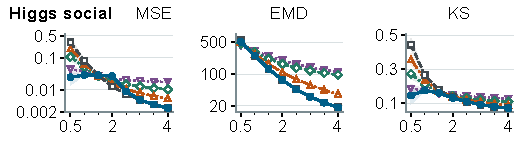
\includegraphics[width=\columnwidth]{icde_sections/figures/gdd_ablation_higgs.pdf}\par
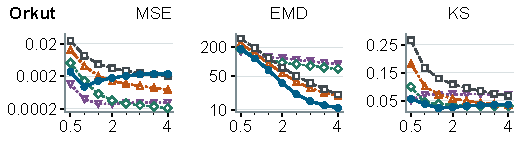
\includegraphics[width=\columnwidth]{icde_sections/figures/gdd_ablation_orkut.pdf}
\caption{Mean ablation errors versus privacy budget $\varepsilon$. Shading: pointwise 95\% bootstrap confidence intervals. MSE and EMD use log scales.}
\label{fig:gdd:en:ablation}
\end{figure}

% \input{icde_sections/figures/e2_wide.tex}  % Compact 3 x 4 double-column plot.
% \input{icde_sections/figures/e2_split.tex} % Two independently floating single-column blocks.

\noindent\textbf{Structural modeling and correction.}
SCRec (without structural correction) sets all seven correction strengths to zero.
On DBLP, enabling correction reduced mean MSE, EMD, and KS at all eight budgets (Fig.~\ref{fig:gdd:en:ablation}).
At $\varepsilon=2$, MSE fell from 0.1272 to 0.01414, EMD from 6.21 to 2.65 (mean paired reduction 3.56, 95\% CI $[3.49,3.63]$), and KS from 0.2755 to 0.0565.
On Orkut, correction reduced EMD and KS at every budget, but increased MSE at $\varepsilon=3.5$ and $4$.
On Bio-DMELA, mean EMD increased at every budget. On Higgs social at $\varepsilon=2$, correction increased MSE from 0.01272 to 0.02728 while reducing KS from 0.1334 to 0.1303.
%Separate reference ablations were available for 411 matched releases. 
On DBLP at $\varepsilon=2$, mean EMD was 2.65 with both references, 4.27 without the $\beta$ reference, and 5.83 without the geometric reference. On Bio-DMELA at the same budget, the corresponding means were 2.03, 2.02, and 1.90. Each of these comparisons used 20 matched runs.
% Removing either reference requires refitting. The independently verified reference-ablation coverage is 411 conditions; contributions vary by network.
 
\noindent\textbf{Learning correction strengths from reports.}
Fixed-0.25, Fixed-0.50, and Fixed-0.75 set each of the seven strengths to the specified value before projection onto the common feasible set in Eq.~\eqref{eq:joint_feasible_domain}.
PrivTDD learns these strengths from the reports using the same references, regions, and correction directions.
Across 32 network--budget settings, its mean error was lower than that of all three presets in 20 settings for EMD, 14 for KS, and seven for MSE.
On Orkut at $\varepsilon=2$, PrivTDD achieved an EMD of 35.58, compared with 57.66 for the best preset on this metric (Fixed-0.25).
On the same reports, Fixed-0.75 attained an MSE of 0.000287 versus 0.001788 for PrivTDD.
%On Bio-DMELA, a preset attained the lowest mean error for each metric at every budget.

\subsection{Sensitivity to the Choice of Regions (E3)}\label{sec:gdd:en:parameters}
% E3: sensitivity to the region partition.
We varied the body, transition, and tail regions used for report-driven distribution correction (Section~\ref{sec:correction}). On all four networks at $\varepsilon\in\{0.5,2\}$, we tested the quantile pairs $(0.80,0.90)$, $(0.90,0.95)$, and $(0.95,0.99)$. The middle pair is the default in E1 and E2. Each pair determines $b_1$ and $b_2$ from the base population distribution conditional on positive triangle degrees. The zero region stays fixed. 
% Vary body, transition, and tail regions using three quantile pairs; keep the zero region fixed. Reuse reports and base fits, refitting only correction strengths. Two Higgs base fits did not converge at epsilon=0.5.
The choice of regions had different effects across networks. Mean EMD varied little on Bio-DMELA and decreased at each step on DBLP at both budgets (Supplementary Material, Section~S3). Figure~\ref{fig:gdd:en:parameters} shows Higgs social and Orkut because raising both quantile levels from the lowest to the highest pair had opposite effects on these networks at $\varepsilon=0.5$. Mean EMD on Higgs social peaked at the default pair, then fell below its value at the lowest pair. On Orkut, it increased at both steps. At $\varepsilon=2$, the default gave the lowest mean EMD on Higgs social. The ordering on Orkut reversed, with mean EMD falling from 42.80 to 29.42 as the two levels increased, while both MSE and KS rose.
% Bio-DMELA EMD changes little; DBLP decreases at both budgets. Higgs and Orkut show opposite low-to-high changes at epsilon=0.5. Higgs is nonmonotone; at epsilon=2, Orkut EMD ordering reverses while MSE and KS rise.
\begin{figure}[htbp]
\centering
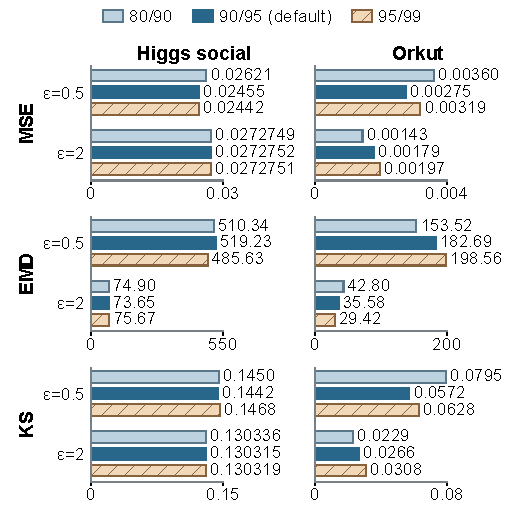
\includegraphics[width=\columnwidth]{icde_sections/figures/e3_sensitivity_means.pdf}
\caption{Sensitivity to the choice of regions on Higgs social and Orkut.}
\label{fig:gdd:en:parameters}
\end{figure}


Triangle-degree is more concentrated on Higgs social, where the top 1\% of nodes by triangle degree account for 47.6\% of the sum of triangle degrees, compared with 32.0\% on Orkut. To locate the errors at $\varepsilon=0.5$, we compared the estimates over the same percentile ranges of each network's true positive triangle-degree distribution. Moving from the lowest to the highest pair increased the EMD contribution between the 90th and 99th percentiles on both networks. On Higgs social, however, it reduced overestimation of the fraction of nodes above extreme triangle-degree thresholds. The EMD contribution above the 99.9th percentile fell in all eight paired runs, by 37.06 on average, and total mean EMD fell by 24.70. On Orkut, the same change worsened underestimation of the fraction of nodes above thresholds in the 90th--99th percentile range. The EMD contribution from this range alone rose by 43.85, close to the total increase of 45.04, and the contribution above the 99.9th percentile also rose.
% The top 1% of nodes carry a larger triangle-degree share on Higgs. Evaluation on fixed true-positive percentile ranges finds increasing 90th--99th percentile error on both networks. Reduced extreme-tail overestimation offsets other errors on Higgs; Orkut underestimation worsens. Truth is used only for evaluation.

\begin{table}[htbp]
\centering
\caption{TDD estimation error by neighbor-pair sampling rate at $\varepsilon=2$.}
% TDD estimation error at different neighbor-pair sampling rates.
\label{tab:gdd:e4:sampling}
\footnotesize
\setlength{\tabcolsep}{2pt}
\renewcommand{\arraystretch}{1.08}
\begin{tabular*}{\columnwidth}{@{\extracolsep{\fill}}lccc@{\hspace{8pt}}ccc@{}}
\toprule
\multirow{2}{*}{\shortstack[l]{Sampling rate}} & \multicolumn{3}{c}{Higgs social} & \multicolumn{3}{c}{Orkut} \\
\cmidrule(lr){2-4}\cmidrule(lr){5-7}
 & MSE & EMD & KS & MSE & EMD & KS \\
\midrule
0.01\% & 0.62058 & 582.89 & 0.5870 & 0.11288 & 945.85 & 0.3288 \\
0.1\% & 0.64318 & 537.15 & 0.5512 & 0.01495 & 2932.84 & 0.2963 \\
1\% & 0.29055 & 661.63 & 0.4008 & 0.13624 & 665.20 & 0.2277 \\
10\% & 0.02011 & 539.99 & 0.1342 & 0.00092 & 199.24 & 0.0453 \\
100\% (E1) & 0.02728 & 73.65 & 0.1303 & 0.00179 & 35.58 & 0.0266 \\
\bottomrule
\end{tabular*}
\end{table}

\subsection{Estimation Accuracy under Neighbor-Pair Sampling (E4)}\label{sec:gdd:en:cost}


On both networks, mean KS decreased at each successive sampling rate, and 10\% sampling gave the lowest mean MSE among the five settings (Table~\ref{tab:gdd:e4:sampling}).
On Higgs social, KS at 10\% sampling was close to that under full enumeration (0.1342 versus 0.1303), although mean EMD remained much higher (539.99 versus 73.65).
On Orkut, mean EMD was 199.24 at 10\% sampling and 35.58 under full enumeration.


% \section{Related Work}
% \noindent\textbf{Private Subgraph Statistics and Distribution Release.}
% Private subgraph analysis studies counts and distributions under different data-access assumptions.
% Centralized methods release triangle-count distributions and common-neighbor histograms over node pairs, assuming a trusted curator with access to the graph~\cite{dingDifferentiallyPrivateTriangle2022,lvPublishingTriangleCounting2021,lvPublishingCommonNeighbors2024a}.
% Day et al.~\cite{day2016degree} use graph projection to publish the degree distribution under central node-DP.
% Local methods use randomized adjacency reports and interaction for subgraph counting and communication reduction~\cite{imola2021locally,LDPGDDImola2022Corrected,guo2026tritr}.
% Related research develops counting error bounds, exploits graph sparsity, and refines per-vertex triangle estimates~\cite{LDPGDDEden2023,mundra2025practical,he2025robust}.
% Wei et al.~\cite{wei2025directed} count cycle and flow triangles in directed graphs under central and local edge-DP.
% Liu et al.~\cite{liu2024relationship} estimate triangle counts from correlated edge observations under $(\varepsilon,\delta)$-edge relationship local differential privacy.
% Other edge-LDP protocols estimate per-edge triangle support for truss decomposition~\cite{zhang2025truss} or count occurrences of acyclic patterns~\cite{hu2026acyclic}.
% PrivTDD targets the TDD from local reports, addressing how count uncertainty propagates through distributional aggregation.

% \noindent\textbf{Frequency and Distribution Estimation under LDP.}
% LDP distribution estimation uses the known randomization mechanism to estimate population frequencies or probability distributions from reports.
% Existing approaches design efficient frequency-estimation protocols~\cite{LDPGDDWang2017,bassily2015succinct} or fit distributions through likelihood models, using smoothing or mixture-component merging to mitigate instability and overfitting~\cite{li2020estimating,ye2025revisiting}.
% These approaches typically start from locally known values, whereas triangle participation depends on edges among neighbors that users cannot directly observe.
% PrivTDD therefore combines private degree and relational reports through an observation model that accounts for neighborhood truncation.

% \noindent\textbf{Structure-Assisted Private Graph Analysis.}
% Structural information assists the estimation of graph metrics and reconstruction of topology from noisy reports.
% Combining private degrees and adjacency information supports graph-metric calibration and Bayesian topology inference~\cite{Ye2022,LDPGDDZhu2023Blink}.
% Structural constraints also enable joint refinement of degree and local triangle targets before graph synthesis~\cite{dong2026ldpgraph}.
% PrivTDD turns models of degree heterogeneity and local clustering into complementary structural references for the degree-conditioned triangle participation distribution, learns regional mass and within-region shape corrections from private reports, and estimates the TDD directly.
\section{Related Work}
\noindent\textbf{Private Subgraph Statistics and Distribution Release.}
Private subgraph analysis studies counts and distributions under different data-access assumptions.
Centralized methods release triangle-count distributions and common-neighbor histograms over node pairs, assuming a trusted curator with access to the graph~\cite{dingDifferentiallyPrivateTriangle2022,lvPublishingTriangleCounting2021,lvPublishingCommonNeighbors2024a}.
Day et al.~\cite{day2016degree} use graph projection to publish the degree distribution under central node-DP.
Local methods use randomized adjacency reports and interaction for subgraph counting and communication reduction~\cite{imola2021locally,LDPGDDImola2022Corrected,guo2026tritr}.
Related research develops counting error bounds, exploits graph sparsity, and refines per-vertex triangle-degree estimates~\cite{LDPGDDEden2023,mundra2025practical,he2025robust}.
Wei et al.~\cite{wei2025directed} count cycle and flow triangles in directed graphs under central and local edge-DP.
Liu et al.~\cite{liu2024relationship} estimate triangle counts from correlated edge observations under $(\varepsilon,\delta)$-edge relationship local differential privacy.
Other edge-LDP protocols estimate the number of triangles containing each edge for truss decomposition~\cite{zhang2025truss} or count occurrences of acyclic patterns~\cite{hu2026acyclic}.
% PrivTDD targets the TDD from local reports, addressing how count uncertainty propagates through distributional aggregation.

\noindent\textbf{Frequency and Distribution Estimation under LDP.}
LDP distribution estimation uses the known randomization mechanism to estimate population frequencies or probability distributions from reports.
Existing approaches design efficient frequency-estimation protocols~\cite{LDPGDDWang2017,bassily2015succinct} or fit distributions through likelihood models, using smoothing or mixture-component merging to mitigate instability and overfitting~\cite{li2020estimating,ye2025revisiting}.
These approaches typically start from locally known values, whereas triangle degrees depend on edges among neighbors that users cannot directly observe.
% PrivTDD therefore combines private degree and relational reports through an observation model that accounts for neighborhood truncation.

\noindent\textbf{Structure-Assisted Private Graph Analysis.}
Structural information assists the estimation of graph metrics and reconstruction of topology from noisy reports.
Combining privatized degree and adjacency reports supports graph-metric calibration and Bayesian topology inference~\cite{Ye2022,LDPGDDZhu2023Blink}.
Structural constraints also enable joint refinement of degree and local triangle-count estimates before graph synthesis~\cite{dong2026ldpgraph}.
% PrivTDD turns models of degree heterogeneity and local clustering into complementary structural references for triangle degrees conditional on node degree, learns regional mass and within-region shape corrections from private reports, and estimates the TDD directly.

\section{Conclusions}
We present PrivTDD for estimating the TDD under edge-local differential privacy.
It decomposes triangle degree into locally known wedge count and an unobserved closure rate, estimates a base distribution from private reports, and adjusts regional probability mass and within-region shape using complementary structural references.
Posterior aggregation retains uncertainty about triangle degrees. Distribution correction and aggregation incur no additional privacy cost.
Experiments on real-world networks validate PrivTDD's distribution estimation and the effectiveness of its key designs.

% Explicit relative path ensures the uploaded ICDE BST is used.
\bibliographystyle{icde_sections/IEEEtran}
% IEEEtran's native last-page column balancing; revisit after content changes.
% \IEEEtriggeratref{20}
\bibliography{icde_sections/references}
% Compile supplementary.tex separately for the extended E1--E3 results.
\end{document}
